
\documentclass[wevj,article,submit,pdftex,moreauthors]{Definitions/mdpi} 
% MDPI internal commands - do not modify
\firstpage{1} 
\makeatletter 
\setcounter{page}{\@firstpage} 
\makeatother
\pubvolume{1}
\issuenum{1}
\articlenumber{0}
\pubyear{2023}
\copyrightyear{2023}
%\externaleditor{Academic Editor: Firstname Lastname}
\datereceived{ } 
\daterevised{ } % Comment out if no revised date
\dateaccepted{ } 
\datepublished{ } 
%\datecorrected{} % For corrected papers: "Corrected: XXX" date in the original paper.
%\dateretracted{} % For corrected papers: "Retracted: XXX" date in the original paper.
\hreflink{https://doi.org/} % If needed use \linebreak
%\doinum{}
%\pdfoutput=1 % Uncommented for upload to arXiv.org

%=================================================================
% Add packages and commands here. The following packages are loaded in our class file: fontenc, inputenc, calc, indentfirst, fancyhdr, graphicx, epstopdf, lastpage, ifthen, float, amsmath, amssymb, lineno, setspace, enumitem, mathpazo, booktabs, titlesec, etoolbox, tabto, xcolor, colortbl, soul, multirow, microtype, tikz, totcount, changepage, attrib, upgreek, array, tabularx, pbox, ragged2e, tocloft, marginnote, marginfix, enotez, amsthm, natbib, hyperref, cleveref, scrextend, url, geometry, newfloat, caption, draftwatermark, seqsplit
% cleveref: load \crefname definitions after \begin{document}

%=================================================================
% Please use the following mathematics environments: Theorem, Lemma, Corollary, Proposition, Characterization, Property, Problem, Example, ExamplesandDefinitions, Hypothesis, Remark, Definition, Notation, Assumption
%% For proofs, please use the proof environment (the amsthm package is loaded by the MDPI class).

%=================================================================
% Full title of the paper (Capitalized)
\Title{A Scalable Approach to Minimize Charging Cost for Electric Bus Fleets}

% MDPI internal command: Title for citation in the left column
\TitleCitation{A Scalable Approach to Minimize Charging Cost for Electric Bus Fleets}

% Author Orchid ID: enter ID or remove command
\newcommand{\orcidauthorA}{0000-0002-7649-4452} % Add \orcidA{} behind the author's name
%\newcommand{\orcidauthorB}{0000-0000-0000-000X} % Add \orcidB{} behind the author's name

% Authors, for the paper (add full first names)
\Author{Daniel Mortensen$^{1}$\orcidA{}, Jacob Gunther$^{2}$}

%\longauthorlist{yes}

% MDPI internal command: Authors, for metadata in PDF
\AuthorNames{Daniel Mortensen, Jacob Gunther}

% MDPI internal command: Authors, for citation in the left column
\AuthorCitation{Mortensen, D.; Gunther, J.}

% Affiliations / Addresses (Add [1] after \address if there is only one affiliation.)
\address{%
$^{1}$ \quad Utah State University; daniel.mortensen@usu.edu \\ 
$^{2}$ \quad  Utah State University; jake.gunther@usu.edu}

% Contact information of the corresponding author
\corres{Correspondence: daniel.mortensen@usu.edu, jake.gunther@usu.edu}

% Current address and/or shared authorship
% The commands \thirdnote{} till \eighthnote{} are available for further notes

%\simplesumm{} % Simple summary

%\conference{} % An extended version of a conference paper

% Abstract (Do not insert blank lines, i.e. \\) 
\begin{abstract}
\textcolor{red}{Insert abstract here}
\end{abstract}

\begin{IEEEkeywords}
\textcolor{red}{Insert keywords here}
\end{IEEEkeywords}

%\abstract{A single paragraph of about 200 words maximum. For research articles, abstracts should give a pertinent overview of the work. We strongly encourage authors to use the following style of structured abstracts, but without headings: (1) Background: place the question addressed in a broad context and highlight the purpose of the study; (2) Methods: describe briefly the main methods or treatments applied; (3) Results: summarize the article's main findings; (4) Conclusions: indicate the main conclusions or interpretations. The abstract should be an objective representation of the article, it must not contain results which are not presented and substantiated in the main text and should not exaggerate the main conclusions.}

% Keywords
%\keyword{keyword 1; keyword 2; keyword 3 (List three to ten pertinent keywords specific to the article; yet reasonably common within the subject discipline.)} 

% The fields PACS, MSC, and JEL may be left empty or commented out if not applicable
%\PACS{J0101}
%\MSC{}
%\JEL{}

%%%%%%%%%%%%%%%%%%%%%%%%%%%%%%%%%%%%%%%%%%
% Only for the journal Diversity
%\LSID{\url{http://}}

%%%%%%%%%%%%%%%%%%%%%%%%%%%%%%%%%%%%%%%%%%
% Only for the journal Applied Sciences
%\featuredapplication{Authors are encouraged to provide a concise description of the specific application or a potential application of the work. This section is not mandatory.}
%%%%%%%%%%%%%%%%%%%%%%%%%%%%%%%%%%%%%%%%%%

%%%%%%%%%%%%%%%%%%%%%%%%%%%%%%%%%%%%%%%%%%
% Only for the journal Data
%\dataset{DOI number or link to the deposited data set if the data set is published separately. If the data set shall be published as a supplement to this paper, this field will be filled by the journal editors. In this case, please submit the data set as a supplement.}
%\datasetlicense{License under which the data set is made available (CC0, CC-BY, CC-BY-SA, CC-BY-NC, etc.)}

%%%%%%%%%%%%%%%%%%%%%%%%%%%%%%%%%%%%%%%%%%
% Only for the journal Toxins
%\keycontribution{The breakthroughs or highlights of the manuscript. Authors can write one or two sentences to describe the most important part of the paper.}

%%%%%%%%%%%%%%%%%%%%%%%%%%%%%%%%%%%%%%%%%%
% Only for the journal Encyclopedia
%\encyclopediadef{For entry manuscripts only: please provide a brief overview of the entry title instead of an abstract.}

%%%%%%%%%%%%%%%%%%%%%%%%%%%%%%%%%%%%%%%%%%
% Only for the journal Advances in Respiratory Medicine
%\addhighlights{yes}
%\renewcommand{\addhighlights}{%

%\noindent This is an obligatory section in “Advances in Respiratory Medicine”, whose goal is to increase the discoverability and readability of the article via search engines and other scholars. Highlights should not be a copy of the abstract, but a simple text allowing the reader to quickly and simplified find out what the article is about and what can be cited from it. Each of these parts should be devoted up to 2~bullet points.\vspace{3pt}\\
%\textbf{What are the main findings?}
% \begin{itemize}[labelsep=2.5mm,topsep=-3pt]
% \item First bullet.
% \item Second bullet.
% \end{itemize}\vspace{3pt}
%\textbf{What is the implication of the main finding?}
% \begin{itemize}[labelsep=2.5mm,topsep=-3pt]
% \item First bullet.
% \item Second bullet.
% \end{itemize}
%}

%%%%%%%%%%%%%%%%%%%%%%%%%%%%%%%%%%%%%%%%%%
\usepackage{bm}
\usepackage{verbatim}
\usepackage{calc}
\usepackage{algorithm2e}
\usepackage{array}
\usepackage{booktabs}
\usepackage{colortbl}
\usepackage{supertabular}
\usepackage{amsmath,amsfonts}
\usepackage{tikz}
\usetikzlibrary{calc}
\usepackage{subfig}
\usepackage{pgfplots} 
\usepackage{pgfplotstable}
\usepgfplotslibrary{patchplots}
\pgfplotsset{compat=1.7}
\usepgfplotslibrary{dateplot}
\usepackage{balance}
\usepackage{ifthen}
\pgfplotsset{
	SmallBarPlot/.style={font=\footnotesize, ybar, width=\linewidth, ymin=0, xmin=0, xmax=1.8, xtick=data, xticklabel style={text width=1.5cm, rotate=0, align=center}},
	SmallTimeSeriesPlot/.style={font=\footnotesize, width=\linewidth, height=2in, date coordinates in=x, xticklabel=\hour:\minute, ymin=0, ymax=100, legend pos=north west,
	major grid style={lightgray}, grid=both, minor grid style={lightgray!25}, minor tick num=1},
	SmallPointPlot/.style={font=\footnotesize, width=\linewidth, legend pos=south west, major grid style={lightgray},
	 grid=both, minor grid style={lightgray!25}, minor tick num=1},
	TimeMatrix/.style={font=\footnotesize, width=\linewidth, height=2in, date coordinates in=x, xticklabel=\hour:\minute} 
	}


\newcommand\makeComparisonBarChartLog[4]{%
	\pgfplotstableread[col sep=comma]{#1}\table
	\begin{tikzpicture}
		\begin{axis}[SmallBarPlot, xticklabels from table={\table}{type}, ylabel=#2, ymode = log]
			\addplot [fill=blue!20, bar width=0.4] table [x expr=\coordindex*0.6 + 1 - 0.1, y=#3]{\table};
			\addplot [fill=red!20, bar width=0.4] table [x expr=\coordindex*0.6 + 1 + 0.1, y=#4]{\table};
		\end{axis}
	\end{tikzpicture} 
}

\newcommand\makeComparisonBarChartThree[5]{%
	\pgfplotstableread[col sep=comma]{#1}\table
	\begin{tikzpicture}
		\begin{axis}[SmallBarPlot, xticklabels from table={\table}{type}, ylabel=#2]
			\addplot [fill=blue!20, bar width=0.15] table [x expr=\coordindex*0.6 + 0.3, y=#3]{\table};
			\addlegendentry{#3}
			\addplot [fill=green!20, bar width=0.15] table [x expr=\coordindex*0.6 + 0.3, y=#4]{\table};
			\addlegendentry{#4}
			\addplot [fill=red!20, bar width=0.15] table [x expr=\coordindex*0.6 + 0.3, y=#5]{\table};
			\addlegendentry{#5}
			\legend{#3, #4, #5}
		\end{axis}
	\end{tikzpicture} 
}

\newcommand\makeComparisonTotalPower[5]{%

\pgfplotstableread[col sep=comma]{#1}\firstTable
\pgfplotstableread[col sep=comma]{#2}\secondTable
\begin{tikzpicture}
	\begin{axis}[SmallTimeSeriesPlot, xlabel=Time (hr:min), ylabel=#3, ymin = -10, ymax=2500, legend style={nodes={scale=0.6}}]
		\filldraw[fill=gray!40, opacity=0.3](625,0) rectangle (917,300);

		\addplot[blue, smooth] table [x = {time}, y = {facilitiesOut}]{\firstTable};
		\addplot[red, smooth] table [x = {time}, y = {facilitiesOut}]{\secondTable};

		\addplot[draw=green!20!black,fill=green!40!cyan!40, mark=pentagon*, only marks, mark size=3pt, y filter/.expression={y==0 ? nan:y}] table [x={time}, y={maxFacilitiesOut}]{\firstTable};
	        \addplot[draw=red,fill=green!10!orange!40, mark=pentagon*, only marks, mark size=3pt, y filter/.expression={y==0 ? nan:y}] table [x={time}, y={maxOnPeakOut}]{\firstTable};

		\addlegendimage{line width=10pt, color=gray!40, draw opacity=0.5}; 
	        \addplot[draw=green!20!black,fill=green!40!cyan!40, mark=pentagon*, only marks, mark size=3pt, y filter/.expression={y==0 ? nan:y}] table [x={time}, y={maxFacilitiesOut}]{\secondTable};
		\addplot[draw=red,fill=green!10!orange!40, mark=pentagon*, only marks, mark size=3pt, y filter/.expression={y==0 ? nan:y}] table [x={time}, y={maxOnPeakOut}]{\secondTable};   

	        \legend{#4, #5, Maximum Overall Average Power, Maximum On-Peak Average Power, On-Peak Time};
	\end{axis} 
\end{tikzpicture}

}

\newcommand\makeComparisonPower[5]{%
	\pgfplotstableread[col sep=comma]{#1}\firstTable
	\pgfplotstableread[col sep=comma]{#2}\secondTable
	\centering
	\begin{tikzpicture}
		\begin{axis}[SmallTimeSeriesPlot, ymin=-10, ymax=800, xlabel=Time (hr:min), ylabel=#3, legend style={nodes={scale=0.7}}]
			\addplot[blue, smooth] table [x = {time}, y = {meanBusPower}]{\firstTable};
			\addplot[red, smooth] table [x = {time}, y = {meanBusPower}]{\secondTable};
			\addplot[brown, smooth] table [x = {time}, y = {loadPower}]{\firstTable};
			\filldraw[fill=gray!40, opacity=0.3](625,0) rectangle (917,950);
			\addlegendimage{line width=10pt, color=gray!40, draw opacity=0.5}
			\legend{#4, #5, Uncontrolled Load, On-Peak Time}
		\end{axis} 
	\end{tikzpicture} 
}


\begin{document}
\section{Introduction} 
\par Battery electric buses (BEBs) are replacing diesel and natural gas buses in public transportation because BEBs offer many benefits \cite{Mahmoud2016} including reduced maintenance \cite{poornesh_comparative_2020}, zero emissions \cite{kato_comparative_2013}, and access to renewable energy \cite{cheng_smart_2020}.  The challenge of prolonged charging times has been addressed in prior research including distributed charging networks \cite{Nimalsiri2020}, bus availability, environmental impact \cite{zhou_bi-objective_2021}, route scheduling \cite{Rinalde_Mixed_2020}, battery health \cite{houbbadi_optimal_2019}, the cost of electricity \cite{Leou_optimal_2017}, and the cost of charging infrastructure \cite{Wei2018}.  
\par Because charge times can be lengthy, some prefer to use high power chargers, which deliver more energy in a smaller period of time. However doing so places large power demands on electrical infrastructure \cite{stahleder_impact_2019} so that power networks becomes unreliable \cite{deb_impact_2017} and expensive because high power requires additional maintenance and upgrades \cite{boonraksa_impact_2019}. An effective charge plan must therefore balance the need to charge quickly with the desire to maintain a low power profile \cite{ojer_development_2020}.  
\par Methods for developing a charge plan range from heuristic approaches \cite{qin_numerical_2016}, to network flow on a graph \cite{whitaker_network_2023}, to reinforcement learning\cite{Wang2019}, to mixed integer linear programs (MILP) \cite{bagherinezhad_spatio-temporal_2020}. Generally, each method minimizes cost by either decreasing the instantaneous power needs for the fleet, or optimizing over time of use tarrifs \cite{He_2019_Fast}.  
\par Scaling these methods to large bus fleets ($>$100 BEBs) and numerous chargers is a challenge due to the size of the problem that must be solved.  For small fleets ($<$50 BEBs) and less than 10 chargers, the optimization problems in \cite{whitaker_network_2023,bagherinezhad_spatio-temporal_2020,He_2019_Fast} have over $10^5$ variables (including binary or integer variables) and over $10^5$ constraints.  Scaling to larger fleets and more chargers leads can stress computational resources and require lengthy solve times.  
\par This paper continues the main theme of prior work which is to develop charging schedules for electric buses that minimize the monthly electricity bill (energy consumption plus power demand) while satisfying route constraints that demand buses to be in specific locations at specific times.  One novelty is that our formulation considers the agregated effects of loading across multiple meters.  While meter agregation is not widespread today, distribution networks must be built to supply worst case loads to each metered circuit.  Therefore, our approach begins to explore how optimization of loads across multilple meters can reduce the overall impact of BEB charging on the grid.  In this work, meter agregation is modeled through the inclusion of uncontrolled (i.e. non-BEB charging) loads.  Specifically, we incorporate historical load data from an electric train (UTA TRAX) that visits a central intermodal hub site in Salt Lake City, Utah which is also a charging stop for BEBs.  
\par The main contribution of the present paper is addressing the matter of scale.  Rather than posing a single large MILP that incorporates every aspect of the charging problem, we solve a series of small subproblems in which the solution to the charging problem becomes successively more refined and moves closer to the optimal schedule.  Our results show that the intermediate subproblems can be solved with a dramatic reduction in runtimes allowing our method to be applied to significantly larger bus fleets.  In a sense, this work explores what is gained in runtime by sacrificing optimality in the schedule.  The subproblems fall into three groups as shown in Fig. \ref{fig:processChain}.  Each sub-problem is solved using a linear, quadratic, or integer program and when used together the series of programs provides a near optimal charge plan. Each sub-problem addresses elements from one of three areas: energy allocation and bus grouping, session length and bus-to-charger assignments, and second-by-second optimization.  

\subsection{Energy Allocation and Group Assignment} 
\par The first set of problems answers two primary questions: At which time should energy be delivered to each bus and which buses' are most able to share chargers and contains three sub-problems: Unconstrained charge schedule, Smooth charge schedule, and group separation.  
\par The unconstrained schedule problem from Section \ref{sec:unconstrainedSchedule} is denoted $p_1$ and computes an optimal charge schedule which minimises the monthly cost of power in the presence of uncontrolled loads under the assumption that each bus maintains a dedicated charger.  
\par The smooth schedule problem from Section \ref{sec:unconstrainedSmoothSchedule} is denoted $p_2$ and has the same form as the unconstrained scheduling problem with two differences: The monthly cost is required to match the optimal cost from the solution to the unconstrained scheduling problem and the objective for the smooth schedule problem penalizes change in the scheduled charge rates.  
\par The group assignment problem from Section \ref{sec:groupAssignment} is denoted $p_3$ and uses the resulting charge schedules from the solution to the smooth schedule problem to separate buses into groups where each bus's schedule overlaps as little as possible with the other schedules for buses in the same group so that each group can be addressed separately to manage the number of computations in succeeding problems.  

\subsection{Session Time and Charger Assignment} 
The problems in the session time and charger assignment section are computed on a per-group basis to reduce the number of computations, address the questions of when should charge sessions start and stop, and on which charger should each session occur and are comprised of three sub-problems: De-Fragmentation, charger assignment, and session refinement.

\par The defragmentation problem from Section \ref{sec:defragmentation} is denoted $p_4$ and attempts to consolidate charge sessions with small amounts of energy to reduce the number of charge sessions and serves to both decrease the computational complexity of the charger assignment problem by reducing the number of charge sessions and simplify the charge schedule to make it more operationally feasible.  
\par After consolidation, each charge session is defined by a minimum/maximum start/stop time as given by the bus's arrival and departure times and an energy requirement in kW. The charger assignment problem from Section \ref{sec:chargerAssignment} is denoted $p_5$ and uses the availability and energy constraints to assign chargers to charge sessions.  
\par Once charge sessions are placed, the final step is to ensure each session makes the most of each charger's availability. Many times, especially when using non-optimal gaps in the charger assignment problem, the charge schedules may not use all available time on a charger. The charger refinement problem is denoted $p_6$ and expands each charge session to fill unused time on either side and prioritizes sessions with higher energy demands for adjacent sessions.  

\subsection{Final Optimization} 
Solutions to the previous problems provide us with a set of charge sessions, energy requirements, and time schedules for specific chargers. The final question to be answered is how should the energy for each session will be delivered. The two sub-problems in the final optimization section mirror the first two problems from the Energy Allocation and Group Assignment section. The first is denoted $p_7$, uses the energy and time constraints from previos solutions to compute an optimal charge schedule in Section \ref{sec:constrainedSchedule} and is analagous to the unconstrained charge problem. The second is denoted $p_8$ and computes a smoothed charge schedule with the same cost as the constrained schedule solution in Section \ref{sec:constrainedSmoothSchedule} and is analagous to the Smooth charge schedule problem in Section \ref{sec:unconstrainedSmoothSchedule}. The table given in Fig. \ref{fig:formulation:features} lists each problem and which features each problem incorporates.

\begin{figure*}\centering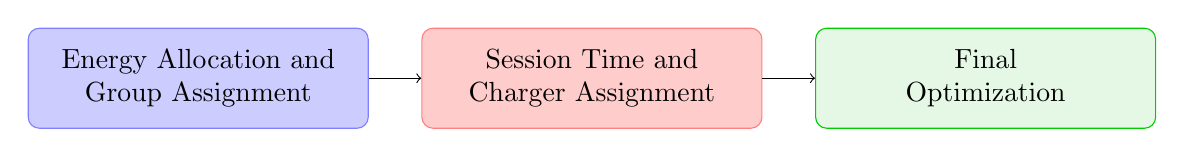
\begin{tikzpicture}
	\node[rectangle, draw=blue!50, fill=blue!20, minimum width=1.7in, minimum height=0.5in, rounded corners](set1) at (0,0) {\begin{tabular}{c} Energy Allocation and\\ Group Assignment\end{tabular}}; 
	\node[rectangle, draw=red!50, fill=red!20, minimum width=1.7in, minimum height=0.5in, rounded corners](set2) at (5,0) {\begin{tabular}{c} Session Time and \\Charger Assignment \end{tabular}}; 
	\node[rectangle, draw=green!80!black, fill=green!70!black!10, minimum width=1.7in, minimum height=0.5in, rounded corners](set3) at (10,0) {\begin{tabular}{c} Final \\ Optimization\end{tabular}}; 
	\draw[->] (set1.east) -- (set2.west);
	\draw[->] (set2.east) -- (set3.west);
\end{tikzpicture}\caption{Overall Processing Chain}\label{fig:processChain}\end{figure*}

 
\begin{figure*}\centering\scalebox{0.8}{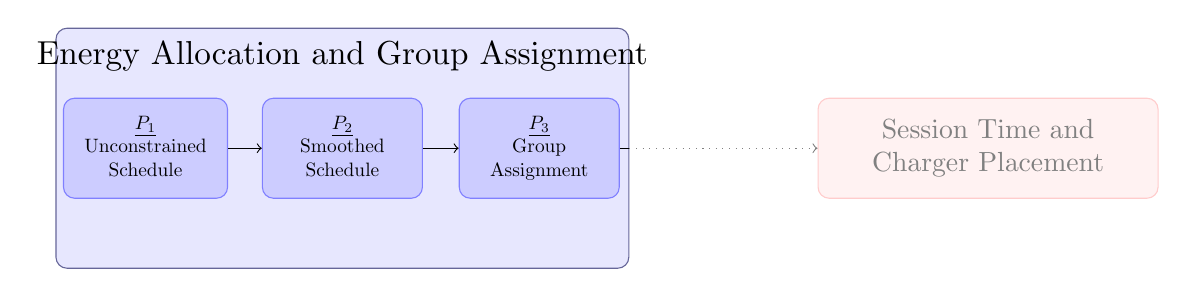
\begin{tikzpicture}
\node[rectangle, draw=gray!80!blue, fill=gray!10!blue!10, minimum width=\textwidth*0.6, minimum height=1.2in, rounded corners, label={[label distance=-0.67cm]above:\scalebox{1.2}{Energy Allocation and Group Assignment}}](outline) at (0,0){};
	\node[rectangle, draw=blue!50, fill=blue!20, minimum width=0.8in, minimum height=0.5in, rounded corners](problem1) at (-2.5,0) {\scalebox{0.7}{\begin{tabular}{c} \underline{$P_1$} \\ Unconstrained \\ Schedule\end{tabular}}}; 
	\node[rectangle, draw=blue!50, fill=blue!20, minimum width=0.8in, minimum height=0.5in, rounded corners](problem2) at (0,0) {\scalebox{0.7}{\begin{tabular}{c}\underline{$P_2$} \\  Smoothed \\ Schedule\end{tabular}}}; 
	\node[rectangle, draw=blue!50, fill=blue!20, minimum width=0.8in, minimum height=0.5in, rounded corners](problem3) at (2.5,0) {\scalebox{0.7}{\begin{tabular}{c}\underline{$P_3$} \\ Group \\ Assignment\end{tabular}}}; 
	\node[rectangle, draw=red!20, fill=red!5, text=black!50, minimum width=1.7in, minimum height=0.5in, rounded corners](problem4) at (8.2,0){\begin{tabular}{c}Session Time and \\ Charger Placement\end{tabular}};
	\draw (problem3.east) -- (outline.east);
	\draw[->, draw=black!50, dotted] (outline.east) -- (problem4.west);
	\draw[->, draw=black] (problem1.east) -- (problem2.west);
	\draw[->, draw=black] (problem2.east) -- (problem3.west);
\end{tikzpicture}}\caption{Processing chain for the energy allocation and group assignment problems} \label{fig:set1Chain}\end{figure*}

 
\begin{figure*}\centering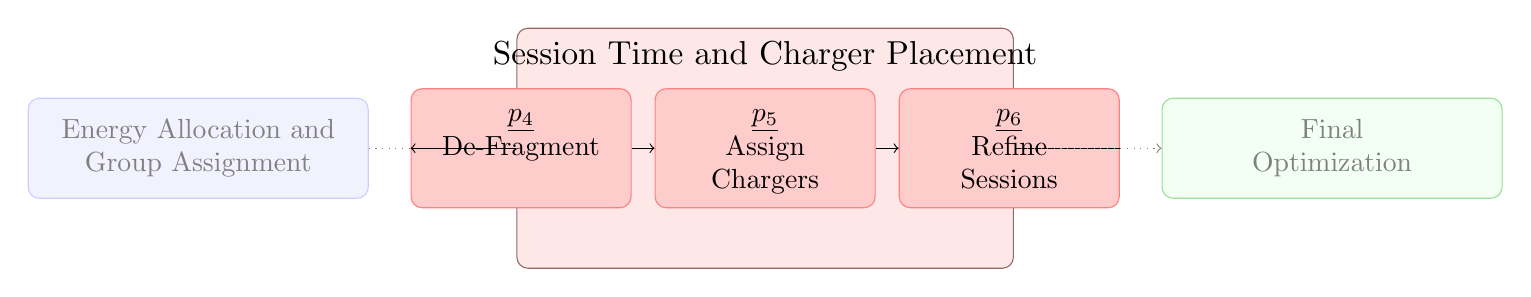
\begin{tikzpicture}
\node[rectangle, draw=gray!80!red, fill=gray!10!red!10, minimum width=\textwidth*0.52, minimum height=1.2in, rounded corners, label={[label distance=-0.67cm]above:\scalebox{1.2}{Session Time and Charger Placement}}](outline) at (0,0){};
	\node[rectangle, draw=red!50, fill=red!20, minimum width=1.1in, minimum height=0.5in, rounded corners](problem1) at (-3.1,0) {\begin{tabular}{c} \underline{$p_4$} \\ De-Fragment \\  \\\end{tabular}}; 
	\node[rectangle, draw=red!50, fill=red!20, minimum width=1.1in, minimum height=0.5in, rounded corners](problem2) at (0,0) {\begin{tabular}{c}\underline{$p_5$} \\ Assign\\ Chargers\end{tabular}}; 
	\node[rectangle, draw=red!50, fill=red!20, minimum width=1.1in, minimum height=0.5in, rounded corners](problem3) at (3.1,0) {\begin{tabular}{c}\underline{$p_6$} \\ Refine\\ Sessions\end{tabular}}; 
	\node[rectangle, draw=blue!20, fill=blue!5, text=black!50, minimum width=1.7in, minimum height=0.5in, rounded corners](problem0) at (-7.2,0){\begin{tabular}{c}Energy Allocation and\\ Group Assignment\end{tabular}};
	\node[rectangle, draw=green!70!black!40, fill=green!5, text=black!50, minimum width=1.7in, minimum height=0.5in, rounded corners](problem4) at (7.2,0){\begin{tabular}{c}Final \\ Optimization\end{tabular}};
	\draw[draw=black!50, dotted] (problem0.east) -- (outline.west);
	\draw[->] (outline.west) -- (problem1.west);
	\draw (problem3.east) -- (outline.east);
	\draw[->, draw=black!50, dotted] (outline.east) -- (problem4.west);
	\draw[->, draw=black] (problem1.east) -- (problem2.west);
	\draw[->, draw=black] (problem2.east) -- (problem3.west);
\end{tikzpicture}\caption{Processing chain for each group} \label{fig:set2Chain}\end{figure*}

 
\begin{figure*}\centering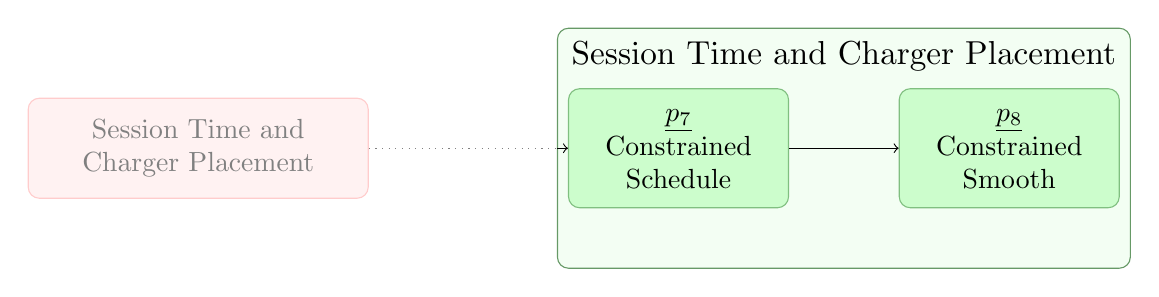
\begin{tikzpicture}
\node[rectangle, draw=gray!80!green, fill=gray!10!green!5, minimum width=\textwidth*0.6, minimum height=1.2in, rounded corners, label={[label distance=-0.67cm]above:\scalebox{1.2}{Session Time and Charger Placement}}](outline) at (0,0){};
	\node[rectangle, draw=green!50!black!50, fill=black!3!green!20, minimum width=1.1in, minimum height=0.5in, rounded corners](problem1) at (-2.1,0) {\begin{tabular}{c} \underline{$p_7$} \\ Constrained \\ Schedule\end{tabular}}; 
	\node[rectangle, draw=green!50!black!50, fill=black!3!green!20, minimum width=1.1in, minimum height=0.5in, rounded corners](problem3) at (2.1,0) {\begin{tabular}{c}\underline{$p_8$} \\ Constrained \\ Smooth\end{tabular}}; 
	\node[rectangle, draw=red!20, fill=red!5, text=black!50, minimum width=1.7in, minimum height=0.5in, rounded corners](problem0) at (-8.2,0){\begin{tabular}{c}Session Time and \\ Charger Placement\end{tabular}};
	\draw[draw=black!50, dotted] (problem0.east) -- (outline.west);
	\draw[->] (outline.west) -- (problem1.west);
	\draw[->, draw=black] (problem1.east) -- (problem3.west);
\end{tikzpicture}\caption{Processing chain for the Final Optimization set} \label{fig:set3Chain}\end{figure*}


\begin{figure*}\label{fig:formulation:features}\centering
\newcommand{\grayhline}{\arrayrulecolor{gray!20} \hline \arrayrulecolor{black}}
\begin{tabular}{l c c c c c c c c}
 Feature                        & $P_1$ & $P_2$ & $P_3$ & $P_4$ & $P_5$ & $P_6$ & $P_7$ & $P_8$ \\ \hline 
Battery State of Charge         &   x   &   x   &       &   x   &       &       &   x   &   x   \\ \grayhline      
Minimize Cost                   &   x   &   x   &       &   x   &       &       &   x   &   x   \\ \grayhline           
Charger Capacity                &   x   &   x   &   x   &   x   &   x   &       &   x   &   x   \\ \grayhline      
Energy Placement                &   x   &   x   &       &   x   &       &       &   x   &   x   \\ \grayhline      
Smooth Charge Plan              &       &   x   &       &       &       &       &       &   x   \\ \grayhline      
Computationally Scalable        &       &       &   x   &       &       &       &   x   &   x   \\ \grayhline      
Small Number of Charge Sessions &       &       &       &   x   &       &       &   x   &   x   \\ \grayhline      
Number of Chargers              &       &       &       &       &   x   &       &   x   &   x   \\ \grayhline      
Efficient Charger Use           &       &       &       &       &       &   x   &   x   &   x   \\ \grayhline      
Precise Charge Plan             &       &       &       &       &       &       &   x   &   x   \\ \grayhline      
\end{tabular} 
\caption{Descriptions of in which problems features are addressed}
\label{fig:formulation:features}
\end{figure*}



%%%%%%%%%%%%%%%%%%%%%%%%%%%%%%%%%%%%%%%%%%
%\section{How to Use this Template}
%
%The template details the sections that can be used in a manuscript. Note that the order and names of article sections may differ from the requirements of the journal (e.g., the positioning of the Materials and Methods section). Please check the instructions on the authors' page of the journal to verify the correct order and names. For any questions, please contact the editorial office of the journal or support@mdpi.com. For LaTeX-related questions please contact latex@mdpi.com.%\endnote{This is an endnote.} % To use endnotes, please un-comment \printendnotes below (before References). Only journal Laws uses \footnote.
%
%% The order of the section titles is different for some journals. Please refer to the "Instructions for Authors” on the journal homepage.
%
%\section{Introduction}
%
%The introduction should briefly place the study in a broad context and highlight why it is important. It should define the purpose of the work and its significance. The current state of the research field should be reviewed carefully and key publications cited. Please highlight controversial and diverging hypotheses when necessary. Finally, briefly mention the main aim of the work and highlight the principal conclusions. As far as possible, please keep the introduction comprehensible to scientists outside your particular field of research. Citing a journal paper \cite{ref-journal}. Now citing a book reference \cite{ref-book1,ref-book2} or other reference types \cite{ref-unpublish,ref-communication,ref-proceeding}. Please use the command \cite{ref-thesis,ref-url} for the following MDPI journals, which use author--date citation: Administrative Sciences, Arts, Econometrics, Economies, Genealogy, Humanities, IJFS, Journal of Intelligence, Journalism and Media, JRFM, Languages, Laws, Religions, Risks, Social Sciences, Literature.
%%%%%%%%%%%%%%%%%%%%%%%%%%%%%%%%%%%%%%%%%%
\section{$P_1$: Unconstrained Schedule \label{sec:unconstrainedSchedule}}

This section describes a program that finds a charge schedule where buses are allowed to charge without regard to the number of available chargers. This solution is considered ``optimal'' and will be used in later sections to formulate a feasible solution that accounts for the actual number of chargers available.

\begin{table*}
\centering
\caption{Description of the billing structure}
\begin{tabular}{c | c c c}
		                   & On-Peak                & Off-Peak               & Facilities (Both)\\ \hline
		Energy Rate        & \$ 0.058282  /kWh & \$ 0.029624 /kWh  & None \\
		Energy Rate Symbol & $\mu_{\text{e-on}}$    & $\mu_{\text{e-off}}$   & None \\ \hline
		Power Rate  & \$ 15.73 /kW           & None                   & \$ 4.81 /kW \\
		Power Rate Symbol  & $\mu_{\text{p-on}}$    & None            & $\mu_{\text{p-all}}$
	\end{tabular}
	\label{tab:charges} 
\end{table*}


\begin{figure*}
\centering
\scalebox{0.8}{
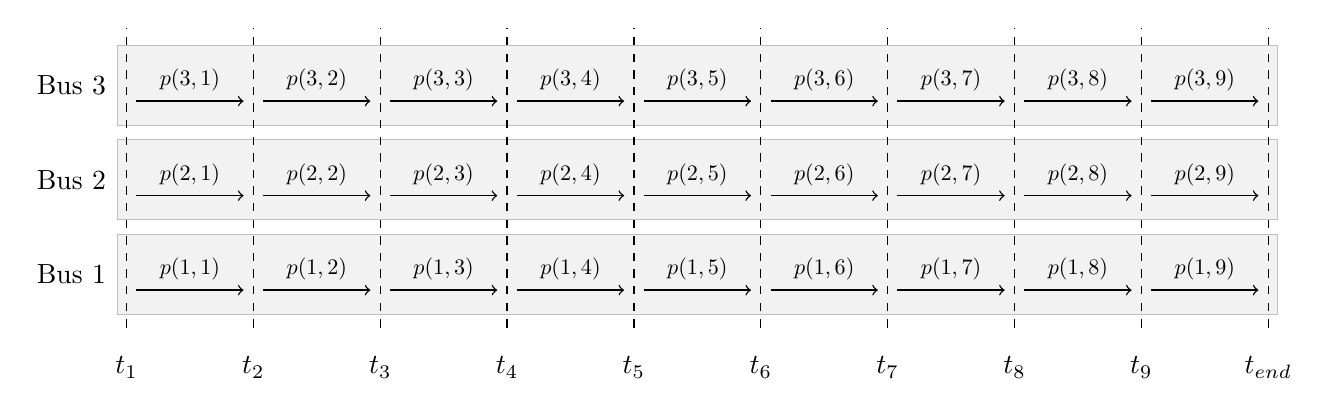
\begin{tikzpicture}
	\node[rectangle, draw=gray!50, fill=gray!10, minimum width=5.8in, minimum height=0.4in](bus1Box) at (7.75,0.8){};
	\node(bus1BoxLabel) at (-0.2, 0.8){Bus 1}; 
	
	\node[rectangle, draw=gray!50, fill=gray!10, minimum width=5.8in, minimum height=0.4in](bus2Box) at (7.75,2){};
	\node(bus1BoxLabel) at (-0.2, 2.0){Bus 2};
	
	\node[rectangle, draw=gray!50, fill=gray!10, minimum width=5.8in, minimum height=0.4in](bus3Box) at (7.75,3.2){};
	\node(bus1BoxLabel) at (-0.2, 3.2){Bus 3};
	
	\foreach \curLab/\preLab[count=\c, evaluate=\c as \pos using {0.5 + (\c - 1)*14.5/9}] in {t_1/t_1, t_2/t_1, t_3/t_2, t_4/t_3, t_5/t_4, t_6/t_7, t_7/t_6, t_8/t_7, t_9/t_8, t_{end}/t_9}
	{
		\node[label=below:$\curLab$](b\c) at (\pos, 0){};
		\node(t) at (\pos, 3.8){};
		\draw[dashed, line width=0.5pt] (b\c.north) -- (t.north); 
		\ifnum\c>1 
			\node(b1Curr) at (\pos, 0.8 - 0.2){};
			\node(b2Curr) at (\pos, 2.0 - 0.2){};
			\node(b3Curr) at (\pos, 3.2 - 0.2){};
			\def\temp{\number\numexpr\c - 1}
			\draw[->, line width=0.5pt] (b1Prev.east) -- node[midway, above]{\scalebox{0.8}{$p(1,\temp)$}}(b1Curr.west);
			\draw[->, line width=0.5pt] (b2Prev.east) -- node[midway, above]{\scalebox{0.8}{$p(2,\temp)$}}(b2Curr.west);
			\draw[->, line width=0.5pt] (b3Prev.east) -- node[midway, above]{\scalebox{0.8}{$p(3,\temp)$}}(b3Curr.west);	
		\fi
			\node(b1Prev) at (\pos, 0.8 - 0.2){};
			\node(b2Prev) at (\pos, 2.0 - 0.2){};
			\node(b3Prev) at (\pos, 3.2 - 0.2){};	
	}
	\path (b9.south) -- node[midway, below=0.1in]{$\hdots$}(b10.south);

\end{tikzpicture}}
\caption{Demonstrates how bus power use is conceptualized}
\label{fig:busPower}
\end{figure*}


\begin{figure*}
\centering
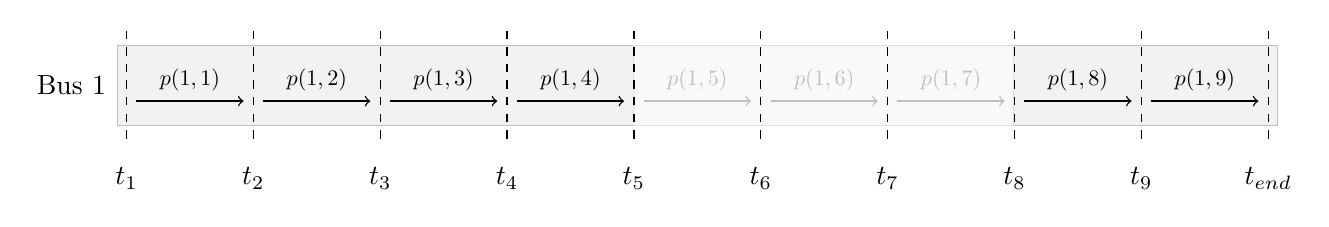
\begin{tikzpicture}
	\node[rectangle, draw=gray!50, fill=gray!10, minimum width=5.8in, minimum height=0.4in](bus1Box) at (7.75,0.8){};
	\node(bus1BoxLabel) at (-0.2, 0.8){Bus 1}; 
	\node[rectangle, draw=gray!25, fill=gray!5, minimum width=1.9in, minimum height=0.4in](bus1Box) at (7.75 + 1.6,0.8){};
	
	\foreach \curLab/\preLab[count=\c, evaluate=\c as \pos using {0.5 + (\c - 1)*14.5/9}] in {t_1/t_1, t_2/t_1, t_3/t_2, t_4/t_3, t_5/t_4, t_6/t_5, t_7/t_6, t_8/t_7, t_9/t_8, t_{end}/t_9}
	{
		\node[label=below:$\curLab$](b\c) at (\pos, 0){};
		\node(t) at (\pos, 1.4){};
		\ifnum\c>1 
			\node(b1Curr) at (\pos, 0.8 - 0.2){};
				\ifnum\c > 5
					\ifnum\c < 9 
						\def\clr{black!25}
					\else
						\def\clr{black}
					\fi
				\else
					\def\clr{black}
				\fi
				\draw[->, line width=0.5pt, \clr] (b1Prev.east) -- node[midway, above]{\scalebox{0.8}{$p(1,\number\numexpr\c-1)$}}(b1Curr.west); 
		\fi
		\node(b1Prev) at (\pos, 0.8 - 0.2){};
		\draw[dashed, line width=0.5pt] (b\c.north) -- (t.north); 
	}
	\path (b9.south) -- node[midway, below=0.1in]{$\hdots$}(b10.south);

\end{tikzpicture}
\caption{Bus schedule with availability}
\label{fig:busAvail}
\end{figure*}



\subsection{Formulation \label{sec:formulation}}

The cost objective we minimize is based on the rate schedule from \cite{rocky_mountain_power_rocky_2021}, which contains two primary elements: the cost of energy and power demand. Energy is billed per kWh using different rates for on-peak and off-peak hours.
%The on-peak rate is more expensive because there is generally more demand for power during this time, whereas off-peak hours tend to be less expensive.
Demand is divided into two components.  The first is a facilities charge which is billed per kW for the highest 15-minute average power use over the course of the month. The second is a demand charge, which is also billed per kW, but is only billed for the highest 15-minute average power usesd during on-peak hours. The rates for each component are given in Table~\ref{tab:charges}.  

Before computing the total monthly cost of electricity, we must define expressions for the average power and energy over time.  Let each day be divided into time intervals of length $\Delta T$ where the average power consumed by bus $i$ during time $j$ is denoted $p(i,j)$ as shown in Fig.~\ref{fig:busPower}. Note that $\Delta T$ may be chosen to be on the order of a second or minute, and expressions for 15-minute averages will be derived later. The solution will yield the average power consumed by each bus during each time interval.

\par The time windows when each bus is available for charging must be accounted for as constraints.  The maximum average power is set to zero when a bus is away from the station. For example, if bus 1 were out on route for times $t_5, t_6,$ and $t_7$, then the average power for those periods would be equal to zero as shown in Fig.~\ref{fig:busAvail}. Let $\bm{b}_{p(i,j)}$ be the average power used by bus $i$ at time index $j$, and $\bm{b}$ be a vector which contains $b_{p(i,j)}$ for each bus and time index. Also let $\mathcal{A} \subset {i\times j}$  be the set of all indices where bus $i$ is in the station during time $t_j$ and let $\tilde{\mathcal{A}}$ be its complement. Also let $p_{\text{max}}$ be the maximum power that a charger can deliver. 
\par The set of constraints that buses do not use power when not in the station are given by
\begin{gather}\label{eqn:obj:power2}
	b_{p(i,j)} = 0 \ \forall i,j \in \tilde{\mathcal{A}}  \\
	0 \leq b_{p(i,j)} \leq p_{\text{max}} \ \forall i,j \in \mathcal{A}
\end{gather}


%%%%%%%%%%%%%%%%%%%%%%%%%%%%%%%%%%%%%%%%%%
\subsection{Battery}
\par Each bus must also maintain its state of charge above acceptable levels throughout the day.  When buses leave the station, each bus discharges some quantity of energy throughout the course of the route. Let $\delta(i,j)$ be the amount of charge lost by bus $i$ at time $j$ and let $h(i,j)$ be the state of charge of bus $i$ at time $j$. The state of charge for each bus can be defined as
\begin{equation}\label{eqn:battery:socPropagation}\begin{aligned}
	h(i,j) &= h(i,j-1) + b_p(i,j - 1)\cdot \Delta T - \delta(i,j) \ \forall i,j>1 \\
	h(i,1) &= \eta_i \ \forall i,
\end{aligned}\end{equation}
where $\eta_i$ is the initial state of charge for bus $i$ and $\Delta T$ is the difference in time between $t_{i,j}$ and $t_{i,j+1}$.
Now that each value for the state of charge is defined, each value for $h$ must be constrained so that it is greater than a given threshold, $h_{\text{min}}$ but does not exceed the maximum battery capacity $h_{\text{max}}$. This yields
\begin{equation} \label{eqn:battery:soc}\begin{aligned}
	-h(i,j) &\le -h_{\text{min}}\ \forall i,j \\
	h(i,j) &\le h_{\text{max}} \ \forall i,j. 
\end{aligned}\end{equation}
\par The final battery related constraint has to do with how we are planning for the bus.  The expenses that come from power are computed monthly, but we desire to simulate the movements of the bus for only a day, and use this to extrapolate what the monthly cost may be.  Therefore, the state of charge for a bus at the end of the day must reflect its starting value.  This yields the following constraint:
\begin{equation}\label{eqn:battery:busPower}
	h_{i,\text{end}} = h(i,1) \ \forall i.
\end{equation}


\subsection{Cumulative Load Management}
\par While this formulation does not directly account for the number of available chargers, we do account for the cumulative load capacities of all chargers.  Let the number of chargers be denoted $n_{\text{charger}}$. We desire to maintain the average cumulative power for each time step at a level that is serviceable given $n_{\text{charger}}$. We define a slack variable $p_c(j)$ which represents the total average power consumed by all buses at time $j$.  The variable $p_c(j)$ is computed as the sum of average bus powers so that
\begin{equation}\label{eqn:cumulative:power}
	p_c(j) = \sum_ib_{p(i,j)}.
\end{equation}


\section{Objective\label{sec:objective}}
\par Now that the relevent constraints have been addressed, we must work towards computing the total objective function. We do so by first computing the total average power for the complete system. This total power is comprised of power used by the buses, and power used by external sources such as lights, ice melt, electric trains, etc which we refer to as ``uncontrolled loads'', where the average power for the uncontrolled loads at time step $j$ is denoted $u(j)$. We compute the total power as the sum of power used by the buses, $p_c(j)$ and the power consumed by uncontrolled loads $u(j)$ so that the total power, denoted $p_t(j)$ is computed as 
\begin{equation*}
	p_t(j) = p_c(j) + u(j)
\end{equation*}
or 
\begin{equation}
	p_t(j) - p_c(j) - u(j) = 0 \ \forall j.
\end{equation}
\par The next step is to compute the fifteen minute average power use for each time step, denoted $p_{\text{15}}$. We do this by letting 
\begin{equation*}
p_{\text{15}}(j) = \frac{1}{n}\sum_{l \in \{j_{15}\}}p_t(l)
\end{equation*}
where $\{j_{15}\}$ is the set of all indices 15 minutes prior to $j$ and $n$ is the cardinality of $\{j_{15}\}$.
Next, note that the rate schedule requires both the maximum overall average power, denoted $p_{\text{facilities}}$, and the maximum average power during on-peak hours, or $p_{\text{demand}}$. Let $\mathcal{S}_{\text{on}}$ be the set of time indices belonging to on-peak hours, and recall that the max over all average power values is greater than or equal to $p_{15}(j)$ for all $j$. We can express this constraint is
\begin{equation*}
	p_{\text{facilities}} \ge p_{15}(j) \ \forall j
\end{equation*}
or alternatively as
\begin{equation}
	p_{15}(j) - p_{\text{facilities}} \le 0 \ \forall j
\end{equation}
Because $p_{\text{facilities}}$ will be used in the objective function, the value for $p_{\text{facilities}}$ will be minimised until it is equal to the largest value in $p_{15}$. Following a similar logic, we also define a set of constraints for the maximum average on-peak power, $p_{\text{demand}}$ so that
\begin{equation}
	p_{15}(i) - p_{\text{demand}} \le 0 \ \forall i \in \mathcal{S}_{\text{on}}
\end{equation}
The next step in computing the objective function is to compute the total {\it energy} consumed during on and off-peak hours respectively.  Let $e_{\text{on}}$ be the total energy consumed during on-peak hours and $e_{\text{off}}$ be the energy consumed during off-peak hours. We can compute energy as the product of average power and time.  In our case, we compute this as 
\begin{equation}\begin{aligned}
	e_{\text{on}} &= \Delta T\cdot \sum_{i \in g}p_t(i) \\ 
	e_{\text{off}} &= \Delta T\cdot \sum_{i \in \tilde{g}}p_t(i) \\ 
\end{aligned}\end{equation}
where $\tilde{g}$ is the complement of $g$. We can now compute the total monthly charge as
\begin{equation}
J_{\text{cost}} = \begin{bmatrix}e_{\text{on}} \\ e_{\text{off}} \\ p_{\text{facilities}} \\ p_{\text{demand}} \end{bmatrix}^T \begin{bmatrix} \mu_{\text{e-on}} \\ \mu_{\text{e-off}} \\ \mu_{\text{p-all}} \\ \mu_{\text{p-on}} \end{bmatrix} 
\end{equation}
Which yields a complete objective function of
\begin{equation}
	J_{\text{all}} = J_{\text{cost}} + J_{\text{thrash}}
\end{equation}



\section{$p_3$: Group Assignment\label{sec:groupAssignment}}
Before the bus charge problem can be solved, we need to address how the problem will scale. In previous attempts to solve the charge problem, routing buses to chargers requires a program which selects an optimal, contention-free schedule by evaluating all possible combinations.
\par Because contention increases on the order of $O(n^2)$ with the number of charge sessions and requires that each combination be evaluated to find an optimal solution, the placement problem is NP-hard \cite{kolesar_branch_1967}. Before we can formulate a scalable solution to the bus problem, we need a method to separate buses into groups to reduce the coupling between charge sessions.
\par The group assignment problem separates buses into $n_{\text{group}}$ groups, where group $m$ is allocated $n^m_{\text{charger}}$ chargers and $n^m_{\text{bus}}$ buses. Each group must have sufficient chargers to fill it's needs and prefer buses with dissimilar schedules to better avoid contention. 
\par We know that the number of cross-terms in future problems will be reduced when each group has the same number of buses. Therefore, let $n^m_{\text{bus}}$ be described as
\begin{equation}\label{eqn:groups:nBusPerGroup}\begin{aligned}
	n^m_{\text{bus}} &\ge \left \lfloor \frac{n_{\text{bus}}}{n_{\text{group}}} \right \rfloor \\
	n^m_{\text{bus}} &\le \left \lceil \frac{n_{\text{bus}}}{n_{\text{group}}} \right \rceil.
\end{aligned}\end{equation}
\par We must also ensure that the number of chargers assigned to each group is exactly equal to the number of available chargers so that
\begin{equation}\label{eqn:groups:nTotalCharger}
	n_{\text{charger}} = \sum_mn_{\text{charger}}^m,
\end{equation}
where $n_{\text{charger}}^m$ is the number of chargers assinged to group $m$.
\par The next set of constraints ensures that each bus is is part of a group exactly once. Let $\beta(i,m)$ be a binary variable which is one when bus $i$ is in group $m$. We constrain each bus to be a member of exactly one group by letting
\begin{equation}\label{eqn:groups:groupId}
	\sum_m\beta(i,m) = 1 \ \forall i.
\end{equation}
\par We must also ensure that buses are assigned to groups where the power delivered to each bus can be achieved with the number of chargers assigned to that group. First, we define a slack variable which gives the total power used in group $m$ at time step $j$ as $p(m,j)$. Recall, we also know the expected power use for each bus as this is a result of $p_1$ as $b_{p(i,j)}$, which allows us to describe the total power for any one group as
\begin{equation}\label{eqn:groups:groupPower}
 p(m,j) = \sum_i\beta(i,m)b_{p(i,j)}.
\end{equation}
\par Next, we know that the total load of each group must be less than or equal to the collective capability of that group's chargers, which can be expressed as
\begin{equation}\label{eqn:groups:chargeLimit}
	n^m_{\text{charger}}\cdot p_{\text{max}} \ge p(m,j) \ \forall m,j
\end{equation}
so that the number of chargers is sufficient to charge the collective load of the group. 
\par We also desire to group buses together who's routes have the least overlap. If two buses contain no overlap, they will be easiest to schedule and the inner product of their schedules from $p_1$ will be equal to zero. Let 
\begin{equation*}
\phi(i,i') = \mathbf{b}(i,:)^T\mathbf{b}(j,:),
\end{equation*}
where $\mathbf{b}(i,:)$ is the charge schedule for bus $i$ as computed in the $p_1$. We desire to minimize the total cross terms $\phi(i,i')$ for all buses in the same group.  Define a slack variable $v(i,i',m)$ which is equal to $\phi(i,i')$ if buses $i$ and $i'$ are both in group $m$ and zero otherwise so that
\begin{equation*}
	\begin{cases}
		v(i,i',m) = \phi(i,i') & \beta(i,m) = 1, \beta(i',m) = 1 \\
		v(i,i',m) = 0 & \text{otherwise},
	\end{cases}
\end{equation*}
which can also be expressed by letting
\begin{equation}\label{eqn:groups:innerProd}\begin{aligned}
	v(i,i',m) &\le \phi(i,i') \\
	v(i,i',m) &\ge \phi(i,i') - M\left (2 - \beta(i,m) - \beta(i',m)\right ) \\
	v(i,i',m) &\le 0 + M\beta(i,m) \\
	v(i,i',m) &\le 0 + M\beta(i',m) \\
	v(i,i',m) &\ge 0.
\end{aligned}\end{equation}
The final objective can then be expressed as
\begin{equation}\label{eqn:groups:objective}
	J_{\text{select}} = \sum_{i,i',m} v(i,i',m).
\end{equation} 
Problems $p_1$ through $p_3$ have yielded preliminary estimates for charge schedules as well as groups into which the buses can be subdivided but have not addressed the problem of fragmentation, where each bus's schedule contains many small charge events where fewer are desired. Before we can address where buses should charge, we must first finalize each bus's charge schedule by decreasing the number of charge events.  
\\[0.1in] \begin{tikzpicture}
	\node[rectangle, rounded corners, fill=gray!8, draw=gray!60, minimum width=\columnwidth, minimum height=0.7in] at (0,0)(box){};
	\node at (0,0.2in)(title){\underline{Summary for $p_3$}};
	\node at ($(box.south)!0.6!(title.south)$)(text){$ 
	\underset{\mathbf{y}}{\text{Min}} \ \eqref{eqn:groups:objective} \ \text{subject to} \ \eqref{eqn:groups:nBusPerGroup} \ \text{--} \ \eqref{eqn:groups:innerProd} % \ \eqref{eqn:groups:nTotalCharger}, \ \eqref{eqn:groups:groupId}, \ \eqref{eqn:groups:groupPower}, \ \eqref{eqn:groups:chargeLimit}, \ \eqref{eqn:groups:innerProd}
$};
\end{tikzpicture}




\section{$P_4$: Defragmentation\label{sec:defragmentation}}

A minimum charge session length is another operational constraint that must be considered. We also consider constraints on minimum energy delivered per session. The intent of these constraints is to avoid charging for short durations or for small amounts of energy so that charge sessions are consolidated for convenience. 

\par To solve these problems, assume there exists a ``smoothed'' solution from $P_2$ which has been appropriately placed in a group from $P_3$. Next, let the preliminary solution be subdivided into charge sessions, each with a specific amount of energy, a minimum start time, and a maximum stop time. If the energy for any charge session is less than the allowed, then this session is marked as ``fragmented''.  The remaining sessions are either marked as ``used'' or ``unused'', where a used session delivers more power than specified by a ``fragmentation-threshold'', and an unused session delivers zero power. 

\par We now propose a new optimization problem in which charge schedule will be defragmented so that each session exceeds a minimum charge threshold. The sessions in question are the ``fragmented'' sessions.  Let $\theta(i,r)$ be a binary variable which indicates if session $r$ from bus $i$ will be active. Because the only sessions in question are fragmented, we only need to define $\theta(i,r)$ for fragmented sessions. Limiting the binary variables in this fashion significantly reduces the computational complexity of this step.  The charge problem will be resolved using the same constraints and objective as in $P_1$, but with the following change. The first change constrains the minimum power delivery for each ``active'' charge session to be {\it at least} as large as the original power delivery from $P_1$. Let $\rho(i,r)$ be a vector which is $\Delta T$, in hours, during the times bus $i$ charges during session $r$ and zero otherwise so that  
\begin{equation}\label{eqn:defragmentation:active}
	\mathbf{b}(i,:)\rho(i,r) \ge \psi(i,j)
\end{equation}
where $\psi(i,j)$ is the minimum energy for session $i,r$ and session $i,r$ is considered ``active''. For inactive sessions, the energy is constrained so that it is equal to zero. Finally, for fragmented sessions, the session energy must be greater than the minimum threshold, $\omega$ when active and zero otherwise which can be expressed as
\begin{equation}\label{eqn:defragmentation:fragmented}\begin{aligned}
	\mathbf{b}(i,:)\rho(i,r) &\ge \omega - \omega(1 - \theta(i,r)) \\
	\mathbf{b}(i,:)\rho(i,r) &\le 0 + \theta(i,r)e_{\text{max}}
\end{aligned}\end{equation}
where $e_{\text{max}}$ is the maximum energy delivered in a session.  The final optimization problem is given below.\\[0.1in]
\begin{tikzpicture}
	\node[rectangle, rounded corners, fill=gray!8, draw=gray!60, minimum width=\columnwidth, minimum height=0.7in] at (0,0)(box){};
	\node at (0,0.2in)(title){\underline{Summary for $P_4$}};
	\node at ($(box.south)!0.6!(title.south)$)(text){$
\underset{\mathbf{y}}{\text{Min}} \ \eqref{sec:unconstrainedSchedule:objective} \ \text{subject to} \ \eqref{eqn:obj:power2} \ \text{--} \ \eqref{eqn:objective:energy}, \ \eqref{eqn:defragmentation:active}, \ \eqref{eqn:defragmentation:fragmented}.
$};
\end{tikzpicture}

\par The solution to the defragmentation problem, $P_4$ provides a charge plan that optimizes the cost of power while requiring that each charge session meet a minimum energy criteria. Up to this point however, we still have not addressed constraints related to the number of chargers which is the focuse of the next section.

% imports
\begin{figure*}
\centering
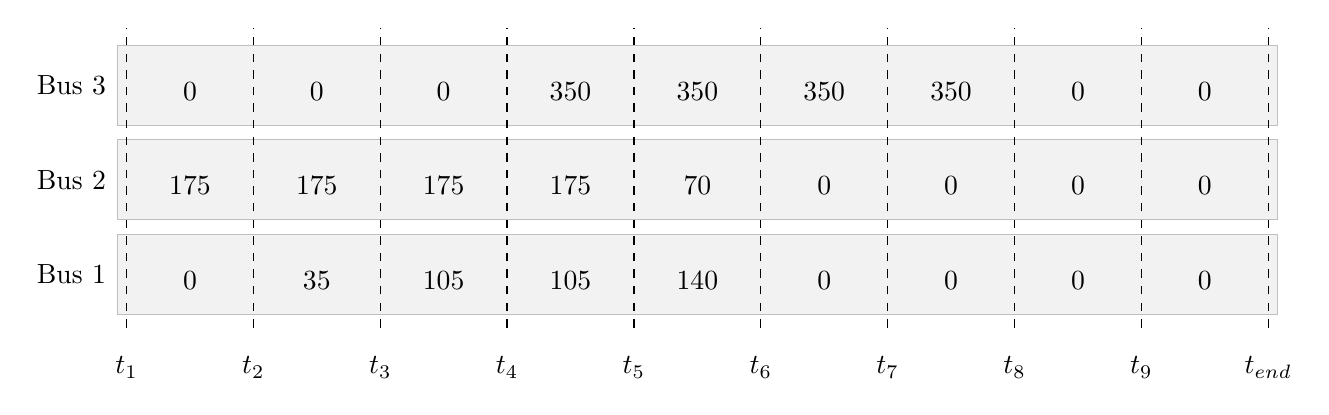
\begin{tikzpicture}
	\node[rectangle, draw=gray!50, fill=gray!10, minimum width=5.8in, minimum height=0.4in](bus1Box) at (7.75,0.8){};
	\node(bus1BoxLabel) at (-0.2, 0.8){Bus 1}; 
	
	\node[rectangle, draw=gray!50, fill=gray!10, minimum width=5.8in, minimum height=0.4in](bus2Box) at (7.75,2){};
	\node(bus1BoxLabel) at (-0.2, 2.0){Bus 2};
	
	\node[rectangle, draw=gray!50, fill=gray!10, minimum width=5.8in, minimum height=0.4in](bus3Box) at (7.75,3.2){};
	\node(bus1BoxLabel) at (-0.2, 3.2){Bus 3};
	
	\foreach \curLab/\preLab[count=\c, evaluate=\c as \pos using {0.5 + (\c - 1)*14.5/9}] in {t_1/t_1, t_2/t_1, t_3/t_2, t_4/t_3, t_5/t_4, t_6/t_7, t_7/t_6, t_8/t_7, t_9/t_8, t_{end}/t_9}
	{
		\node[label=below:$\curLab$](b\c) at (\pos, 0){};
		\node(t) at (\pos, 3.8){};
		\draw[dashed, line width=0.5pt] (b\c.north) -- (t.north); 
		\ifnum\c>1 
			\node(b1Curr) at (\pos, 0.8 - 0.2){};
			\node(b2Curr) at (\pos, 2.0 - 0.2){};
			\node(b3Curr) at (\pos, 3.2 - 0.2){};
			\path(b1Prev.east) -- node(node1\c)[midway, above]{}(b1Curr.west);
			\path(b2Prev.east) -- node(node2\c)[midway, above]{}(b2Curr.west);
			\path(b3Prev.east) -- node(node3\c)[midway, above]{}(b3Curr.west);	
		\fi
			\node(b1Prev) at (\pos, 0.8 - 0.2){};
			\node(b2Prev) at (\pos, 2.0 - 0.2){};
			\node(b3Prev) at (\pos, 3.2 - 0.2){};	
	}
	\path (b9.south) -- node[midway, below=0.1in]{$\hdots$}(b10.south);
	\node at (node12.center){0};
	\node at (node13.center){35};
	\node at (node14.center){105};
	\node at (node15.center){105};
	\node at (node16.center){140};
	\node at (node17.center){0};
	\node at (node18.center){0};
	\node at (node19.center){0};
	\node at (node110.center){0};
	\node at (node22.center){175};
	\node at (node23.center){175};
	\node at (node24.center){175};
	\node at (node25.center){175};
	\node at (node26.center){70};
	\node at (node27.center){0};
	\node at (node28.center){0};
	\node at (node29.center){0};
	\node at (node210.center){0};
	\node at (node32.center){0};
	\node at (node33.center){0};
	\node at (node34.center){0};
	\node at (node35.center){350};
	\node at (node36.center){350};
	\node at (node37.center){350};
	\node at (node38.center){350};
	\node at (node39.center){0};
	\node at (node310.center){0};

\end{tikzpicture}
\caption{An example solution to a 3-bus, 2-charger scenario from $p_4$}
\label{fig:solutionExample}
\end{figure*}

\begin{figure*}
\centering
\scalebox{0.8}{
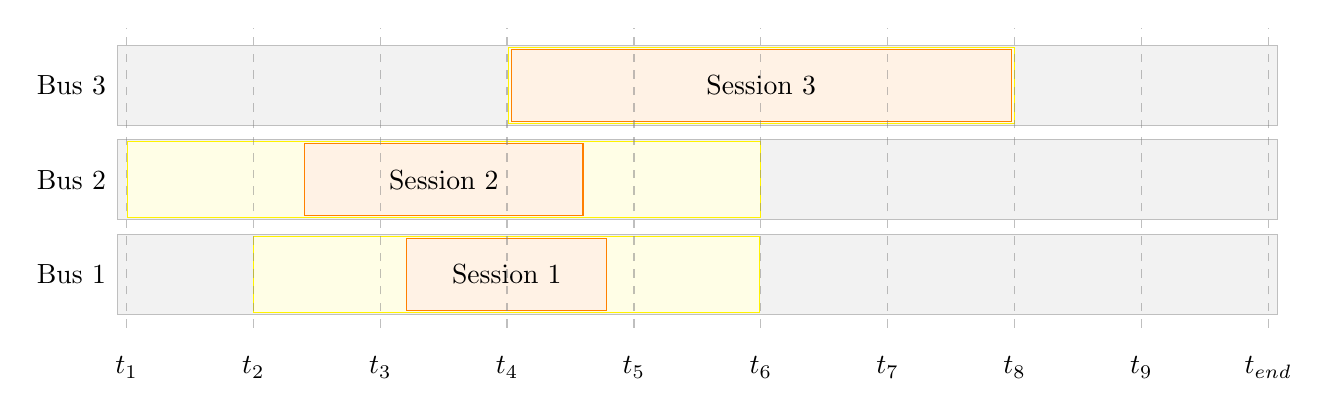
\begin{tikzpicture}
	\node[rectangle, draw=gray!50, fill=gray!10, minimum width=5.8in, minimum height=0.4in](bus1Box) at (7.75,0.8){};
	\node(bus1BoxLabel) at (-0.2, 0.8){Bus 1}; 
	\node[rectangle, draw=yellow!100, fill=yellow!10, minimum width=2.53in, minimum height=0.38in](charge11) at (5.33, 0.8){};
	\node[rectangle, draw=orange!100, fill=orange!10, minimum width=1in, minimum height=0.36in](charge111) at (5.33, 0.8){Session 1};

	\node[rectangle, draw=gray!50, fill=gray!10, minimum width=5.8in, minimum height=0.4in](bus2Box) at (7.75,2){};
	\node(bus1BoxLabel) at (-0.2, 2.0){Bus 2};
	\node[rectangle, draw=yellow!100, fill=yellow!10, minimum width=3.1625in, minimum height=0.38in](charge11) at (4.53, 2){};
	\node[rectangle, draw=orange!100, fill=orange!10, minimum width=1.3915in, minimum height=0.36in](charge111) at (4.53, 2){Session 2};
	
	\node[rectangle, draw=gray!50, fill=gray!10, minimum width=5.8in, minimum height=0.4in](bus3Box) at (7.75,3.2){};
	\node(bus1BoxLabel) at (-0.2, 3.2){Bus 3}; 
	\node[rectangle, draw=yellow!100, fill=yellow!10, minimum width=2.53in, minimum height=0.38in](charge11) at (8.56, 3.2){};
	\node[rectangle, draw=orange!100, fill=orange!10, minimum width=2.50in, minimum height=0.36in](charge111) at (8.56, 3.2){Session 3};


	\foreach \curLab/\preLab[count=\c, evaluate=\c as \pos using {0.5 + (\c - 1)*14.5/9}] in {t_1/t_1, t_2/t_1, t_3/t_2, t_4/t_3, t_5/t_4, t_6/t_7, t_7/t_6, t_8/t_7, t_9/t_8, t_{end}/t_9}
		{
			\node[label=below:$\curLab$](b\c) at (\pos, 0){};
			\node(t) at (\pos, 3.8){};
			\draw[dashed, line width=0.5pt, black!50, opacity=0.5] (b\c.north) -- (t.north); 
		}
		\path (b9.south) -- node[midway, below=0.1in]{$\hdots$}(b10.south); 
\end{tikzpicture}}
\caption{Demonstrates how results from $p_4$ can be reexpressed in terms of continuous variables} 
\label{fig:refactorExample}
\end{figure*}



\begin{figure*}
\centering
\scalebox{0.8}{
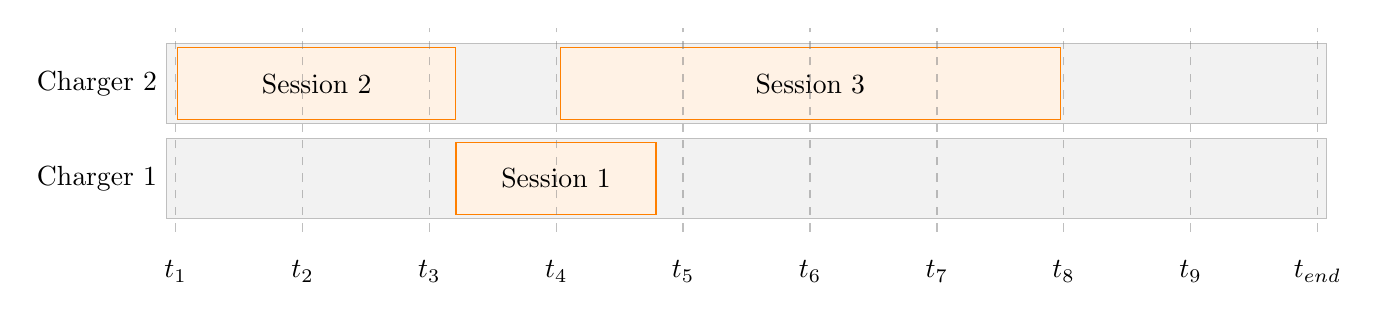
\begin{tikzpicture}
	\node[rectangle, draw=gray!50, fill=gray!10, minimum width=5.8in, minimum height=0.4in](bus1Box) at (7.75,0.8){};
	\node(bus1BoxLabel) at (-0.5, 0.8){Charger 1}; 

	\node[rectangle, draw=gray!50, fill=gray!10, minimum width=5.8in, minimum height=0.4in](bus2Box) at (7.75,2){};
	\node(bus1BoxLabel) at (-0.5, 2.0){Charger 2};
	\node[rectangle, draw=orange!100, fill=orange!10, minimum width=1.3915in, minimum height=0.36in](charge111) at (2.29, 2){Session 2}; 
	\node[rectangle, draw=orange!100, fill=orange!10, minimum width=1in, minimum height=0.36in](charge111) at (5.33, 0.8){Session 1};
	\node[rectangle, draw=orange!100, fill=orange!10, minimum width=2.50in, minimum height=0.36in](charge111) at (8.56, 2){Session 3};


	\foreach \curLab/\preLab[count=\c, evaluate=\c as \pos using {0.5 + (\c - 1)*14.5/9}] in {t_1/t_1, t_2/t_1, t_3/t_2, t_4/t_3, t_5/t_4, t_6/t_7, t_7/t_6, t_8/t_7, t_9/t_8, t_{end}/t_9}
		{
			\node[label=below:$\curLab$](b\c) at (\pos, 0){};
			\node(t) at (\pos, 2.58){};
			\draw[dashed, line width=0.5pt, black!50, opacity=0.5] (b\c.north) -- (t.north); 
		}
		\path (b9.south) -- node[midway, below=0.1in]{$\hdots$}(b10.south); 
\end{tikzpicture}}
\caption{Demonstrates the solution to $p_5$}
\label{fig:secondSolutionExample}
\end{figure*}



\begin{figure*}
\centering
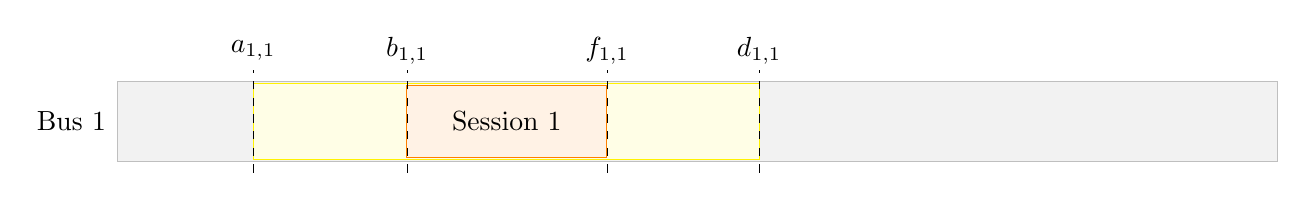
\begin{tikzpicture}
	\node[rectangle, draw=gray!50, fill=gray!10, minimum width=5.8in, minimum height=0.4in](bus1Box) at (7.75,0.8){};
	\node(bus1BoxLabel) at (-0.2, 0.8){Bus 1}; 
	\node[rectangle, draw=yellow!100, fill=yellow!10, minimum width=2.53in, minimum height=0.38in](charge11) at (5.33, 0.8){};
	\node[rectangle, draw=orange!100, fill=orange!10, minimum width=1in, minimum height=0.36in](charge111) at (5.33, 0.8){Session 1}; 
	\draw[dashed] (0.83in,0.15) -- (0.83in,1.45);
	\node at (0.83in,1.7){$a_{1,1}$};
	\draw[dashed] (3.36in, 0.15) -- (3.36in, 1.45);
	\node at (3.36in,1.7){$d_{1,1}$};
	\draw[dashed] (1.6in, 0.15) -- (1.6in, 1.45);
	\node at (1.6in,1.7){$b_{1,1}$};
	\draw[dashed] (2.6in, 0.15) -- (2.6in, 1.45);
	\node at (2.6in,1.7){$f_{1,1}$};
\end{tikzpicture}
\caption{Gives variables of optimization for $p_5$}
\label{fig:secondProgramVars}
\end{figure*} 


\section{$p_5$: Charger Assignment\label{sec:chargerAssignment}}
The results from $p_4$ give a general estimate of how much and when buses should charge, however we must still address two primary issues. The first is defining concrete start and stop times for each charge session. The second is limiting the charge sessions to a finite number of chargers. 
\par Consider a solution to a three bus, two charger scenario given in Fig. \ref{fig:solutionExample}.
Note that there appears to be three buses charging at the same time from $t_5$ to $t_6$ even though there are only two chargers.  We can reformulate this solution in terms of continuous start and stop variables and a variable charge rate so that the {\it duration} of each charge session may be relaxed. The objective is to store the given energy in the corresponding bus within the given charge interval.  
\par Note how few of the charge sessions utilize the chargers to full capacity. This implies that there exists a smaller charge window in which equivalent power can be delivered. This allow us to use the charge durations from the solution from Fig. \ref{fig:solutionExample} as bounds on {\it allowable} charge windows instead of absolute truth. 
\par An example of how Fig. \ref{fig:solutionExample} may be reformulated is given in Fig. \ref{fig:refactorExample}. Note how the actual charge sessions don't necessarily need to take up all the time they were initially allocated in the first solution and that these times can fluctuate if the average charge rate is less than the maximum charger capacity. In this example, we assume a maximum charge capacity of 350kW.  
\par Note how the third charge session does have to be exactly where it was scheduled because the average is equal to the maximum charge rate.
If we examine just the schedule for Bus 1, we note that there are four essential variables for the corresponding charge session: $a(i,r)$, $b(i,r)$, $f(i,r)$ and $d(i,r)$ which represent the minimum start time, actual start time, actual end time, and maximum end time respectively. 
\par The problem we must now solve is one of arranging these ``rectangles'' such that each one is larger than it's minimum width (or charge time).  We must also account for the number of chargers. It can be helpful to view the problem as a bin packing problem, where each session must fit within the ``swim lane'' of a charger.  For example, taking the charge sessions given in Fig. \ref{fig:refactorExample} and arranging them so that there is no overlap between sessions will yield a valid solution as shown in Fig. \ref{fig:secondSolutionExample}.
\par From Fig. \ref{fig:secondProgramVars}, we know that $a(i,r), b(i,r),f(i,r)$ and $d(i,r)$ must be such that 
\begin{equation}\label{eqn:assignment:eqn1}\begin{aligned}
	a(i,r) \le b(i,r) \\
	b(i,r) \le f(i,r) \\
	f(i,r) \le d(i,r), 	
\end{aligned}\end{equation}
where $a(i,r)$ and $d(i,r)$ are known from the previous optimization problem, and $b(i,r)$ and $f(i,r)$ are optimization variables. 
\par We must differentiate between chargers and so, define $\sigma(i,r,k)$ as a binary selector variable which is one if charger $k$ services bus $i$ for session $r$ and zero otherwise. We know that only one charger can charge each bus at a time. We also know that each charge session {\it must} be serviced, which implies that
\begin{equation}\label{eqn:assignment:eqn2}
	\sum_k \sigma(i,r,k) = 1  \ \forall i,r.
\end{equation}
\par Next, we also know that during each session a certain amount of energy must be transferred from the charger to the battery.  The amount of energy that must be transferred to bus $i$ during session $r$ are given in the solution to $p_4$ and are denoted $e(i,r)$. We can compute a minimum time window from these values by letting 
\begin{equation}\label{eqn:assignment:eqn3}
	w(i,r)_{\text{min}} = \frac{e(i,r)}{p_\text{max}}.
\end{equation}
If we include constraints for a minimum time per session, then the previous expression becomes
\begin{equation*}
	w(i,r)_{\text{min}} = \text{max}\left ( w_{\text{min}}, \frac{e(i,r)}{p_\text{max}} \right ).
\end{equation*}
\par Because this is the minimum time window, we must ensure that the difference between the start and stop times is at least this large so that
\begin{equation}\label{eqn:assignment:eqn4}
	f(i,r) - b(i,r) \ge w(i,r) \ \forall i,r.
\end{equation}
\par The final set of constraints deals with contention so that no charger can be scheduled for two sessions that overlap. let $\mathcal{L} = \{(i,r)\times (i',r') \}$ where charge sessions $i,r$ and $i',r'$ have the potential to overlap. Before we can prevent overlap, we must define a binary variable $l(i,r,i',r')$ which is equal to one when session $i,r$ is scheduled before session $i',r'$ and zero otherwise so that
\begin{equation}
	\begin{cases}
		f(i,r) \le b(i',r') & l(i,r,i',r') = 1 \\
		f(i',r') \le b(i',r') & l(i,r,i',r') = 0. 
	\end{cases}
\end{equation}
Here we can expand this thought through use of the ``big-M'' technique.  Let $M$ be large. In this case, we can set it equal to the number of seconds in a day. We know what the top constraint must be trivially satisfied when $l(i,r,i',r') = 0$ and the bottom must also when $l(i,r,i',r') = 1$.  This leads to a reformulation so that
\begin{equation*}\begin{aligned}
		f(i,r) - b(i',r') & \le M(1 - l(i,r,i',r')\\
		f(i',r') - b(i,r) & \le l(i,r,i',r')M.  
\end{aligned}\end{equation*}
However, this constraint {\it only} needs to hold when sessions $i,r$ and $i',r'$ are scheduled to charge on the same charger or that $\sigma(i,r,k) = \sigma(i',r',k) = 1$. We can reformulate the above constraint to satisfy this condition by letting
\begin{equation}\label{eqn:assignment:eqn5}\begin{aligned}
	f(i,r) - b(i',r') & \le M(3 - \sigma(i,r,k) - \sigma(i',r',k) - l(i,r,i',r')) \\
	f(i',r') - b(i,r) & \le M(2 - \sigma(i,r,k) - \sigma(i',r',k) + l(i,r,i',r')).
\end{aligned}\end{equation}
\par Finally, we desire the schedule to closely match the charge plan from $p_4$, which occurs when each charge session matches the durations given in $p_4$ and so we formulated an objective function which minimizes the differences in the given plan and the results from $p_4$ by letting the objective be
\begin{equation}\label{eqn:assignment:eqn6}
	\underset{f,b}{\text{min}} \sum_{i,r}\lVert b(i,r) - a(i,r)\rVert_2^2 + \lVert f(i,r) - d(i,r) \rVert_2^2,
\end{equation}
which has the effect of driving each variable to the desired value and more heavily penalizing values that are further from their optimal.
\par Ideally, when $p_5$ is solved to optimality, the chargers are fully utilized. However, optimality for $p_5$ is computationally demanding and scalable solutions may require relaxations in the optimality gap so that time on the chargers is not fully utilized. The next section uses the ordering from $p_5$, but recomputes session start/stop times to better utilize the charger availability even when sub-optimal gaps are given for $p_5$.
\\[0.1in] \begin{tikzpicture}
	\node[rectangle, rounded corners, fill=gray!8, draw=gray!60, minimum width=\columnwidth, minimum height=0.7in] at (0,0)(box){};
	\node at (0,0.2in)(title){\underline{Summary for $p_5$}};
	\node at ($(box.south)!0.6!(title.south)$)(text){$
	\underset{\mathbf{y}}{\text{Min}} \ \eqref{eqn:assignment:eqn6} \ \text{subject to} \ \eqref{eqn:assignment:eqn1} \ \text{--} \ \eqref{eqn:assignment:eqn5}.
$};
\end{tikzpicture} 

\section{$p_6$: Optimizing Charge Schedules\label{sec:optimizingChargeSchedules}}
Many times it is not feasible to compute the optimal set of charge schedules given in the previous sections. As the number of buses and charge sessions becomes large, computing a small-MIPGap solution becomes intractable. Using a large MIPGap resolves issues related to computational complexity, but results in sub-optimal charge-time windows.
\par We compute a more optimal set of charge windows by using the results from $p_5$ to infer charger assignment, and ordering for each charge session. We also know that the optimal solution will expand the charge windows to use any available time where a charger is unused, implying that the ``stop'' time for each session will either be equal to it's buse's departure time, or the start time of the next window which can be expressed as
\begin{equation}\label{eqn:optChargeSchedules:eqn1}
\begin{cases}
	c(s,i,r+1) = c(f,i,r) & c(d,i,r) > c(a,i,r+1)\\[0.08in]
	\begin{aligned}
	c(s,i,r+1) &= c(a,i,r+1) \\
	c(f,i,r) &= c(d,i,r)
	\end{aligned} & c(d,i,r) <= c(a,i,r+1), 
\end{cases}
\end{equation}
where $c(s,i,r)$ is the start time for charger $i$'s $r^{\text{th}}$ charge session, $c(f,i,r)$ is the stop time for charger $i$'s $r^{\text{th}}$ charge session, $c(d,i,r)$ is the departure time for the bus scheduled for charger $i$'s $r^{\text{th}}$ charge session, and $c(a,i,r)$ is the arrival time for the bus scheduled for charger $i$'s $r^{\text{th}}$ charge session. 
The minimum charge length must also be used so that energy can be properly delivered, so that
\begin{equation}\label{eqn:optChargeSchedules:eqn2}
	c(f,i,r) - c(s,i,r) \ge w(i,r),
\end{equation}
where $w(i,r)$ is the corresponding minimum charge time corresponding the session.
\par The final step to optimizing the charge windows is to give preference to windows with larger power deliveries. Let the objective for the optimization program be 
\begin{equation}\label{eqn:optChargeSchedule:objective}
	J_{\text{window}} = \frac{1}{n}\sum_{i,r} \left \lVert \frac{c(f,i,r) - c(s,i,r)}{e(i,r)} \right \rVert^2_2.
\end{equation}
When the function $J$ contains windows with equal amounts of energy, the minimum will be found where each charge interval is the same width. As the amount of energy increases, the objective penalizes less for larger window sizes and thus gives preference to high energy sessions.
\par Now each charge session is assigned to a charger so that contention for limited chargers has been managed for each group. Furthermore, each session also specifies target energy requirements which manage the risks of depleting batteries but does not give instructions on how the energy is to be delivered. The energy delivery problem is addressed in $p_7$ and combined results for all groups so that the charge schedule begins to approach a more global solution.  
\\[0.1in] \begin{tikzpicture}
	\node[rectangle, rounded corners, fill=gray!8, draw=gray!60, minimum width=\columnwidth, minimum height=0.7in] at (0,0)(box){};
	\node at (0,0.2in)(title){\underline{Summary for $p_5$}};
	\node at ($(box.south)!0.6!(title.south)$)(text){$ 
	\underset{\mathbf{y}}{\text{Min}} \ \eqref{eqn:optChargeSchedule:objective} \ \text{subject to} \ \eqref{eqn:optChargeSchedules:eqn1}, \ \eqref{eqn:optChargeSchedules:eqn2}
$};
\end{tikzpicture} 



\section{$P_7:$ Constrained Schedule\label{sec:constrainedSchedule}}
Up to this point, we have computed a near-optimal schedule which assumes any bus can charge without regard to the number of chargers. We then separated buses into groups to reduce the scale of the problem and treat each sub-problem separately while we defragment sessions and assign each charge session to specific chargers before determining the final start and stop times for each bus's charge session.
\par The final step in this process is to determine how the energy will be delivered so that cost is minimised. We begin with constraints for bus power, energy, and cost from Section \ref{sec:unconstrainedSchedule} that are expressed as equations \eqref{eqn:obj:power2}, \eqref{eqn:battery:busPower}, \eqref{eqn:objective:pt}, \eqref{eqn:objective:p15}, \eqref{eqn:objective:pFac}, \eqref{eqn:objective:pDem} and \eqref{eqn:objective:energy}. Next, include constraints for energy so that the energy for each charge session is properly delivered using a modified version of \eqref{eqn:defragmentation:active} so that
\begin{equation}\label{eqn:constrainedSchedule:modified}
	\mathbf{b}(i,:)\rho(i,r) = \psi(i,r),
\end{equation}
where $\psi(i,r)$ is the required energy for bus $i$ during rest period $r$ as computed from the solution of the defragmentation problem.  The resulting optimization problem is given below.\\[0.1in]
\begin{tikzpicture}
	\node[rectangle, rounded corners, fill=gray!8, draw=gray!60, minimum width=\columnwidth, minimum height=0.7in] at (0,0)(box){};
	\node at (0,0.2in)(title){\underline{Summary for $P_7$}};
	\node at ($(box.south)!0.6!(title.south)$)(text){$
	\underset{\mathbf{y}}{\text{Min}} \ \eqref{sec:unconstrainedSchedule:objective} \ \text{subject to} \ \eqref{eqn:obj:power2}, \ \eqref{eqn:battery:busPower}, \ \eqref{eqn:objective:pt} \ \text{--} \ \eqref{eqn:objective:energy}, \ \eqref{eqn:constrainedSchedule:modified}
$};
\end{tikzpicture}

\section{$P_8:$ Constrained Smooth Schedule\label{sec:constrainedSmoothSchedule}}
 \par The charge schedule from $P_7$ will contain the same on-off switching defects as the solution to $P_1$ which can be managed as before by executing $P_7$ once again with the same modifications that lead to $P_2$: (1) constrain the cost terms in the objective to equal their values from $P_7$, and (2) reduce the difference of sequential charge rates with the smoothing objective from \ref{eqn:objective:smooth}.  The resulting optimization problem is given below.\\[0.1in] \begin{tikzpicture}
	\node[rectangle, rounded corners, fill=gray!8, draw=gray!60, minimum width=\columnwidth, minimum height=0.7in] at (0,0)(box){};
	\node at (0,0.2in)(title){\underline{Summary for $P_8$}};
	\node at ($(box.south)!0.6!(title.south)$)(text){$
	\underset{\mathbf{y}}{\text{Min}} \ \eqref{eqn:objective:smooth} \ \text{subject to} \ \eqref{eqn:obj:power2}, \ \eqref{eqn:battery:busPower}, \ \eqref{eqn:objective:pt} \ \text{--} \ \eqref{eqn:objective:energy}, \ \eqref{eqn:unconstrainedSmooth:equivalence}, \ \eqref{eqn:constrainedSchedule:modified}
$};
\end{tikzpicture}

\section{Results}
The results given in this section aim to demonstrate how the proposed method can be used to find a scalable solution to the bus charge problem. Because the proposed solution contains various sub-problems, optimization parameters for each sub-problem may be tuned to best meet the demands of a given scenario, allowing for a wide degree of flexibility that is not present in prior works which formulate solutions to the bus charge problem as a single program.
\subsection{Overall Performance}
In this section, we compare the proposed method with a baseline algorithm and a method developed by \cite{he_battery_2022} The baseline method models how bus drivers charge their electric vehicles at the Utah Transit Authority in Salt Lake City, Utah. At UTA, when bus drivers arrive at the station, they refuel their electric buses whenever a charger is available so that the number of charge sessions is maximized. The method from \cite{he_battery_2022} works somewhat differently by minimizing the cost of energy with respect to the time of use tariffs $\mu_{e-on}$ and $\mu_{e-off}$.
\par The comparison we observe is given for a 10-bus, 10-charger scenario and a single group. Each method was used to compute a charge schedule and the costs from demand, facilities, and energy charges are given in Fig. \ref{fig:results:costComparison}. Note how the baseline algorithm suffers significantly from the demand charges associated with On-Peak Power, and \cite{he_battery_2022} incurs additional cost from the facilities charges, indicating that an emphasis on energy charges and habitual charging patterns can be improved.
\par We observe where the differences in cost originate in Fig. \ref{fig:results:totalPower}. Observe how the baseline charge profile achieved the largest 15-minute average power between 19:12 and 21:36 which is during on-peak hours and consequently yielded the large On-Peak Power charges given in Fig. \ref{fig:results:costComparison}. Additionally, note how the proposed method maintains a relatively flat power profile so that the load is balanced throughout the day which we investigate in Fig. \ref{fig:results:powerPlot}.
\par In Fig. \ref{fig:results:powerPlot}, note how the proposed method produces a bus load that mirrors the uncontrolled load, yielding the flat load profile from Fig. \ref{fig:results:totalPower} which is especially prevalent from 7:12 to 14:24. The results show that the proposed method works well, outperforming both historical patterns at UTA as well and improves upon prior academic techniques.
\begin{figure}
	\centering
	\makeComparisonBarChartThree{media/11_results/costComparison.csv}{Cost (Dollars)}{Baseline}{He et al.}{Proposed}
	\caption{Cost comparison with prior work}
	\label{fig:results:costComparison}
\end{figure} 

 
\begin{figure*}
	\centering
	\makeComparisonPower{media/11_results/powerPlotfiscal.csv}{media/11_results/powerPlotconsumption.csv}{15-Minute Average Power (kW)}{Proposed}{He et al.}
	\caption{Comparison between uncontrolled and bus loads}
	\label{fig:results:powerPlot}
\end{figure*}


\begin{figure*}
	\centering
	\makeComparisonTotalPower{media/11_results/totalPowerfiscalproTime.csv}{media/11_results/totalPowerconsumptionproTime.csv}{15-Minute Average Power (kW)}{Proposed}{He et al.}
	\caption{15-Minute average power for one day}
	\label{fig:results:totalPower}
\end{figure*}


\subsection{Optimality Gaps and Contention}
In the previous section, we discussed performance of the proposed method when each program is solved to an optimal solution. In general, the most computationally demanding solution addressed bus-to-charger placement and generally requires a gap of $1\times10^{-5}$ for optimality. This work also seeks to address how to compute a solution in a scalable manner and so this section reviews computational time as the number of buses increases.  
\par This section considers a 7-charger scenario and compares runtime results for 8, 9, and 10 buses to illustrate how runtimes for set optimality gaps change as contention increases. Fig. \ref{fig:results:scalabilityTimeVsGap} shows how the computational time increases as the optimality gap decreases. Note how the computational time suddenly increases as the gap decreases, a phenomena which is exacerbated as contention increases. Additionally, note that the optimality gaps are small even before the sudden increase in runtime indicating that it may not be necessary to solve past the turning point where the runtime suddenly increases. 
\begin{figure}
\centering
\begin{tikzpicture}
	\pgfplotstableread[col sep=comma]{\rootdirectorythree/media/11_results/avgPowerVsDurationOpt.csv}\tableOpt
	\pgfplotstableread[col sep=comma]{\rootdirectorythree/media/11_results/avgPowerVsDurationDis.csv}\tableDis
	\begin{axis}[ylabel=Duration (Seconds), xlabel=Average Power (kWh), ymode=log]
		\addplot[blue!20, draw=blue, only marks,mark size=1pt] table[x=avgPower, y=duration] {\tableOpt};
		\addplot[red!20, draw=red, only marks,mark size=1pt] table[x=avgPower, y=duration] {\tableDis};
		\legend{Optimal Solution, Relaxed Optimality Gap}
	\end{axis}
\end{tikzpicture}
\caption{Comparison of charge session duration vs average charge rate}
\label{fig:results:sessionComparison}
\end{figure}
 
\begin{figure}
	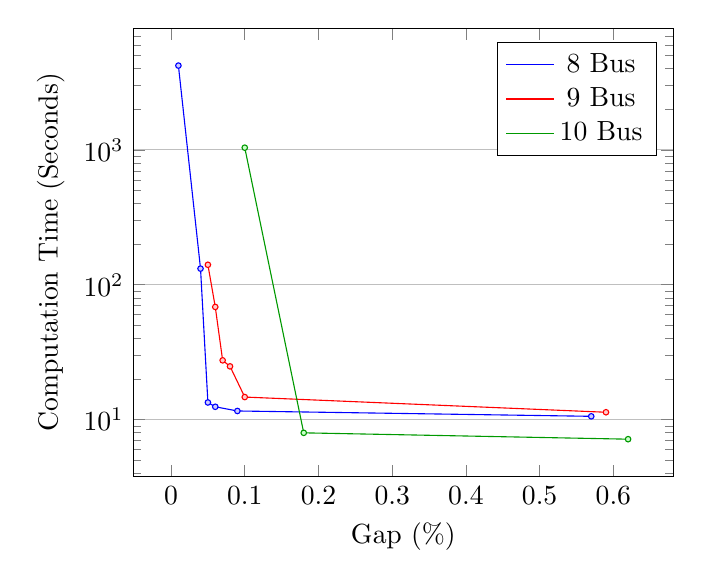
\begin{tikzpicture}
		\begin{axis}[ymajorgrids=true, ylabel={Computation Time (Seconds)}, ymode=log, xlabel={Gap (\%)}, legend pos=north east]%, xtick={0.1, 0.05, 0.01, 0.005, 0.001, 0.0005, 0.0001, 0.00005, 0.00001, 0.000005, 0.000001}, xticklabels={$1\times10^{-1}$, $5\times10^{-2}$, $1\times10^{-2}$, $5\times10^{-3}$, $1\times10^{-3}$, $5\times10^{-4}$, $1\times10^{-4}$, $5\times10^{-5}$, $1\times10^{-5}$, $5\times10^{-6}$, $1\times10^{-6}$}]
			\addplot[blue] coordinates {
				(0.57, 10.58)
				(0.09, 11.59)
				(0.06, 12.45)
				(0.05, 13.40)
				(0.04, 131.78)
				(0.01, 4223.25)
			};
			\addplot[red] coordinates {
				(0.59, 11.34)
				(0.10, 14.70)
				(0.08, 24.83)
				(0.07, 27.51)
				(0.06, 68.49)
				(0.05, 140.70)
			};
			\addplot[green!60!black] coordinates {
				(0.62, 7.16)
				(0.18, 7.98)
				(0.10, 1039.33)
			}; 
			\addplot[fill=blue!20, draw=blue, only marks, mark size=1pt] coordinates {
				(0.57, 10.58)
				(0.09, 11.59)
				(0.06, 12.45)
				(0.05, 13.40)
				(0.04, 131.78)
				(0.01, 4223.25)}; 
			\addplot[fill=red!20, draw=red, only marks, mark size=1pt] coordinates {
				(0.59, 11.34)
				(0.10, 14.70)
				(0.08, 24.83)
				(0.07, 27.51)
				(0.06, 68.49)
				(0.05, 140.70)
			}; 
			\addplot[fill=green!20, draw=green!60!black, only marks, mark size=1pt] coordinates{
				(0.62, 7.16)
				(0.18, 7.98)
				(0.10, 1039.33) 
			};
	\legend{8 Bus, 9 Bus, 10 Bus};
		\end{axis}
	\end{tikzpicture}
	\caption{Comparison of Runtime for a 7-Charger Scenario}
	\label{fig:results:scalabilityTimeVsGap}
\end{figure}



\subsection{Contention: Sub-Optimal Schedules}
In the previous section we observed that the proposed method cannot scale with contention if the optimality gap dips below the turning point where runtime suddenly increases. In this section, we show that a relaxed optimality gap in the charger placement problem may result in an undesirable solution and consequently that there exist scenarios that require small optimality gaps which normally lie beyond the turning point shown in Fig. \ref{fig:results:scalabilityTimeVsGap}, indicating the need to reduce the charger assignment problem's computational complexity. 
\par Fig. \ref{fig:results:sessionComparison} displays the charge session durations as a function of average charge rate for two 18 bus 6 charger scenarios where the first was computed using a small optimality gap and the second resulted when the gap was relaxed. Note how the charge sessions from the optimal solution tend to have larger session durations and lower charge rates than the relaxed solution which is desired because sessions with low charge rates and long durations are simpler to carry out in practice. 
\par Figures \ref{fig:results:disoptimalRoutes} and \ref{fig:results:optimalRoutes} show the corresponding optimal and relaxed charge plans by letting the color at the $i,j$ location represent the charge rate for bus $i$ at time $j$ and show why an optimal solution to the charger assignment problem yields better charge sessions. Observe how the first sessions for buses 1 -- 4 and 6 -- 13 are assigned to a single charger in the relaxed solution, which compresses the charge sessions to accommodate the large number of buses while the remaining chargers appear to have one session at most. In comparison, the optimal solution in Fig. \ref{fig:results:optimalRoutes} has a more evenly distributed session load for each charger so that each session is lengthened, leading to lower charge rates. 
\par It is also interesting to note that the monthly costs of each solution may or may not be equivalent even though an optimal solution is clearly superior. Therefore, a small gap is required to consistently achieve optimal session placement. We also know from Fig. \ref{fig:results:scalabilityTimeVsGap} that small optimality gaps may increase the number of computations so that the charger assignment problem becomes intractable for large numbers of buses.  
\pgfplotsset{
	ChargeSessionImage/.style={colormap={mymap}{[1pt] rgb(0pt)=(0.2422,0.1504,0.6603); rgb(1pt)=(0.2444,0.1534,0.6728); rgb(2pt)=(0.2464,0.1569,0.6847); rgb(3pt)=(0.2484,0.1607,0.6961); rgb(4pt)=(0.2503,0.1648,0.7071); rgb(5pt)=(0.2522,0.1689,0.7179); rgb(6pt)=(0.254,0.1732,0.7286); rgb(7pt)=(0.2558,0.1773,0.7393); rgb(8pt)=(0.2576,0.1814,0.7501); rgb(9pt)=(0.2594,0.1854,0.761); rgb(11pt)=(0.2628,0.1932,0.7828); rgb(12pt)=(0.2645,0.1972,0.7937); rgb(13pt)=(0.2661,0.2011,0.8043); rgb(14pt)=(0.2676,0.2052,0.8148); rgb(15pt)=(0.2691,0.2094,0.8249); rgb(16pt)=(0.2704,0.2138,0.8346); rgb(17pt)=(0.2717,0.2184,0.8439); rgb(18pt)=(0.2729,0.2231,0.8528); rgb(19pt)=(0.274,0.228,0.8612); rgb(20pt)=(0.2749,0.233,0.8692); rgb(21pt)=(0.2758,0.2382,0.8767); rgb(22pt)=(0.2766,0.2435,0.884); rgb(23pt)=(0.2774,0.2489,0.8908); rgb(24pt)=(0.2781,0.2543,0.8973); rgb(25pt)=(0.2788,0.2598,0.9035); rgb(26pt)=(0.2794,0.2653,0.9094); rgb(27pt)=(0.2798,0.2708,0.915); rgb(28pt)=(0.2802,0.2764,0.9204); rgb(29pt)=(0.2806,0.2819,0.9255); rgb(30pt)=(0.2809,0.2875,0.9305); rgb(31pt)=(0.2811,0.293,0.9352); rgb(32pt)=(0.2813,0.2985,0.9397); rgb(33pt)=(0.2814,0.304,0.9441); rgb(34pt)=(0.2814,0.3095,0.9483); rgb(35pt)=(0.2813,0.315,0.9524); rgb(36pt)=(0.2811,0.3204,0.9563); rgb(37pt)=(0.2809,0.3259,0.96); rgb(38pt)=(0.2807,0.3313,0.9636); rgb(39pt)=(0.2803,0.3367,0.967); rgb(40pt)=(0.2798,0.3421,0.9702); rgb(41pt)=(0.2791,0.3475,0.9733); rgb(42pt)=(0.2784,0.3529,0.9763); rgb(43pt)=(0.2776,0.3583,0.9791); rgb(44pt)=(0.2766,0.3638,0.9817); rgb(45pt)=(0.2754,0.3693,0.984); rgb(46pt)=(0.2741,0.3748,0.9862); rgb(47pt)=(0.2726,0.3804,0.9881); rgb(48pt)=(0.271,0.386,0.9898); rgb(49pt)=(0.2691,0.3916,0.9912); rgb(50pt)=(0.267,0.3973,0.9924); rgb(51pt)=(0.2647,0.403,0.9935); rgb(52pt)=(0.2621,0.4088,0.9946); rgb(53pt)=(0.2591,0.4145,0.9955); rgb(54pt)=(0.2556,0.4203,0.9965); rgb(55pt)=(0.2517,0.4261,0.9974); rgb(56pt)=(0.2473,0.4319,0.9983); rgb(57pt)=(0.2424,0.4378,0.9991); rgb(58pt)=(0.2369,0.4437,0.9996); rgb(59pt)=(0.2311,0.4497,0.9995); rgb(60pt)=(0.225,0.4559,0.9985); rgb(61pt)=(0.2189,0.462,0.9968); rgb(62pt)=(0.2128,0.4682,0.9948); rgb(63pt)=(0.2066,0.4743,0.9926); rgb(64pt)=(0.2006,0.4803,0.9906); rgb(65pt)=(0.195,0.4861,0.9887); rgb(66pt)=(0.1903,0.4919,0.9867); rgb(67pt)=(0.1869,0.4975,0.9844); rgb(68pt)=(0.1847,0.503,0.9819); rgb(69pt)=(0.1831,0.5084,0.9793); rgb(70pt)=(0.1818,0.5138,0.9766); rgb(71pt)=(0.1806,0.5191,0.9738); rgb(72pt)=(0.1795,0.5244,0.9709); rgb(73pt)=(0.1785,0.5296,0.9677); rgb(74pt)=(0.1778,0.5349,0.9641); rgb(75pt)=(0.1773,0.5401,0.9602); rgb(76pt)=(0.1768,0.5452,0.956); rgb(77pt)=(0.1764,0.5504,0.9516); rgb(78pt)=(0.1755,0.5554,0.9473); rgb(79pt)=(0.174,0.5605,0.9432); rgb(80pt)=(0.1716,0.5655,0.9393); rgb(81pt)=(0.1686,0.5705,0.9357); rgb(82pt)=(0.1649,0.5755,0.9323); rgb(83pt)=(0.161,0.5805,0.9289); rgb(84pt)=(0.1573,0.5854,0.9254); rgb(85pt)=(0.154,0.5902,0.9218); rgb(86pt)=(0.1513,0.595,0.9182); rgb(87pt)=(0.1492,0.5997,0.9147); rgb(88pt)=(0.1475,0.6043,0.9113); rgb(89pt)=(0.1461,0.6089,0.908); rgb(90pt)=(0.1446,0.6135,0.905); rgb(91pt)=(0.1429,0.618,0.9022); rgb(92pt)=(0.1408,0.6226,0.8998); rgb(93pt)=(0.1383,0.6272,0.8975); rgb(94pt)=(0.1354,0.6317,0.8953); rgb(95pt)=(0.1321,0.6363,0.8932); rgb(96pt)=(0.1288,0.6408,0.891); rgb(97pt)=(0.1253,0.6453,0.8887); rgb(98pt)=(0.1219,0.6497,0.8862); rgb(99pt)=(0.1185,0.6541,0.8834); rgb(100pt)=(0.1152,0.6584,0.8804); rgb(101pt)=(0.1119,0.6627,0.877); rgb(102pt)=(0.1085,0.6669,0.8734); rgb(103pt)=(0.1048,0.671,0.8695); rgb(104pt)=(0.1009,0.675,0.8653); rgb(105pt)=(0.0964,0.6789,0.8609); rgb(106pt)=(0.0914,0.6828,0.8562); rgb(107pt)=(0.0855,0.6865,0.8513); rgb(108pt)=(0.0789,0.6902,0.8462); rgb(109pt)=(0.0713,0.6938,0.8409); rgb(110pt)=(0.0628,0.6972,0.8355); rgb(111pt)=(0.0535,0.7006,0.8299); rgb(112pt)=(0.0433,0.7039,0.8242); rgb(113pt)=(0.0328,0.7071,0.8183); rgb(114pt)=(0.0234,0.7103,0.8124); rgb(115pt)=(0.0155,0.7133,0.8064); rgb(116pt)=(0.0091,0.7163,0.8003); rgb(117pt)=(0.0046,0.7192,0.7941); rgb(118pt)=(0.0019,0.722,0.7878); rgb(119pt)=(0.0009,0.7248,0.7815); rgb(120pt)=(0.0018,0.7275,0.7752); rgb(121pt)=(0.0046,0.7301,0.7688); rgb(122pt)=(0.0094,0.7327,0.7623); rgb(123pt)=(0.0162,0.7352,0.7558); rgb(124pt)=(0.0253,0.7376,0.7492); rgb(125pt)=(0.0369,0.74,0.7426); rgb(126pt)=(0.0504,0.7423,0.7359); rgb(127pt)=(0.0638,0.7446,0.7292); rgb(128pt)=(0.077,0.7468,0.7224); rgb(129pt)=(0.0899,0.7489,0.7156); rgb(130pt)=(0.1023,0.751,0.7088); rgb(131pt)=(0.1141,0.7531,0.7019); rgb(132pt)=(0.1252,0.7552,0.695); rgb(133pt)=(0.1354,0.7572,0.6881); rgb(134pt)=(0.1448,0.7593,0.6812); rgb(135pt)=(0.1532,0.7614,0.6741); rgb(136pt)=(0.1609,0.7635,0.6671); rgb(137pt)=(0.1678,0.7656,0.6599); rgb(138pt)=(0.1741,0.7678,0.6527); rgb(139pt)=(0.1799,0.7699,0.6454); rgb(140pt)=(0.1853,0.7721,0.6379); rgb(141pt)=(0.1905,0.7743,0.6303); rgb(142pt)=(0.1954,0.7765,0.6225); rgb(143pt)=(0.2003,0.7787,0.6146); rgb(144pt)=(0.2061,0.7808,0.6065); rgb(145pt)=(0.2118,0.7828,0.5983); rgb(146pt)=(0.2178,0.7849,0.5899); rgb(147pt)=(0.2244,0.7869,0.5813); rgb(148pt)=(0.2318,0.7887,0.5725); rgb(149pt)=(0.2401,0.7905,0.5636); rgb(150pt)=(0.2491,0.7922,0.5546); rgb(151pt)=(0.2589,0.7937,0.5454); rgb(152pt)=(0.2695,0.7951,0.536); rgb(153pt)=(0.2809,0.7964,0.5266); rgb(154pt)=(0.2929,0.7975,0.517); rgb(155pt)=(0.3052,0.7985,0.5074); rgb(156pt)=(0.3176,0.7994,0.4975); rgb(157pt)=(0.3301,0.8002,0.4876); rgb(158pt)=(0.3424,0.8009,0.4774); rgb(159pt)=(0.3548,0.8016,0.4669); rgb(160pt)=(0.3671,0.8021,0.4563); rgb(161pt)=(0.3795,0.8026,0.4454); rgb(162pt)=(0.3921,0.8029,0.4344); rgb(163pt)=(0.405,0.8031,0.4233); rgb(164pt)=(0.4184,0.803,0.4122); rgb(165pt)=(0.4322,0.8028,0.4013); rgb(166pt)=(0.4463,0.8024,0.3904); rgb(167pt)=(0.4608,0.8018,0.3797); rgb(168pt)=(0.4753,0.8011,0.3691); rgb(169pt)=(0.4899,0.8002,0.3586); rgb(170pt)=(0.5044,0.7993,0.348); rgb(171pt)=(0.5187,0.7982,0.3374); rgb(172pt)=(0.5329,0.797,0.3267); rgb(173pt)=(0.547,0.7957,0.3159); rgb(175pt)=(0.5748,0.7929,0.2941); rgb(176pt)=(0.5886,0.7913,0.2833); rgb(177pt)=(0.6024,0.7896,0.2726); rgb(178pt)=(0.6161,0.7878,0.2622); rgb(179pt)=(0.6297,0.7859,0.2521); rgb(180pt)=(0.6433,0.7839,0.2423); rgb(181pt)=(0.6567,0.7818,0.2329); rgb(182pt)=(0.6701,0.7796,0.2239); rgb(183pt)=(0.6833,0.7773,0.2155); rgb(184pt)=(0.6963,0.775,0.2075); rgb(185pt)=(0.7091,0.7727,0.1998); rgb(186pt)=(0.7218,0.7703,0.1924); rgb(187pt)=(0.7344,0.7679,0.1852); rgb(188pt)=(0.7468,0.7654,0.1782); rgb(189pt)=(0.759,0.7629,0.1717); rgb(190pt)=(0.771,0.7604,0.1658); rgb(191pt)=(0.7829,0.7579,0.1608); rgb(192pt)=(0.7945,0.7554,0.157); rgb(193pt)=(0.806,0.7529,0.1546); rgb(194pt)=(0.8172,0.7505,0.1535); rgb(195pt)=(0.8281,0.7481,0.1536); rgb(196pt)=(0.8389,0.7457,0.1546); rgb(197pt)=(0.8495,0.7435,0.1564); rgb(198pt)=(0.86,0.7413,0.1587); rgb(199pt)=(0.8703,0.7392,0.1615); rgb(200pt)=(0.8804,0.7372,0.165); rgb(201pt)=(0.8903,0.7353,0.1695); rgb(202pt)=(0.9,0.7336,0.1749); rgb(203pt)=(0.9093,0.7321,0.1815); rgb(204pt)=(0.9184,0.7308,0.189); rgb(205pt)=(0.9272,0.7298,0.1973); rgb(206pt)=(0.9357,0.729,0.2061); rgb(207pt)=(0.944,0.7285,0.2151); rgb(208pt)=(0.9523,0.7284,0.2237); rgb(209pt)=(0.9606,0.7285,0.2312); rgb(210pt)=(0.9689,0.7292,0.2373); rgb(211pt)=(0.977,0.7304,0.2418); rgb(212pt)=(0.9842,0.733,0.2446); rgb(213pt)=(0.99,0.7365,0.2429); rgb(214pt)=(0.9946,0.7407,0.2394); rgb(215pt)=(0.9966,0.7458,0.2351); rgb(216pt)=(0.9971,0.7513,0.2309); rgb(217pt)=(0.9972,0.7569,0.2267); rgb(218pt)=(0.9971,0.7626,0.2224); rgb(219pt)=(0.9969,0.7683,0.2181); rgb(220pt)=(0.9966,0.774,0.2138); rgb(221pt)=(0.9962,0.7798,0.2095); rgb(222pt)=(0.9957,0.7856,0.2053); rgb(223pt)=(0.9949,0.7915,0.2012); rgb(224pt)=(0.9938,0.7974,0.1974); rgb(225pt)=(0.9923,0.8034,0.1939); rgb(226pt)=(0.9906,0.8095,0.1906); rgb(227pt)=(0.9885,0.8156,0.1875); rgb(228pt)=(0.9861,0.8218,0.1846); rgb(229pt)=(0.9835,0.828,0.1817); rgb(230pt)=(0.9807,0.8342,0.1787); rgb(231pt)=(0.9778,0.8404,0.1757); rgb(232pt)=(0.9748,0.8467,0.1726); rgb(233pt)=(0.972,0.8529,0.1695); rgb(234pt)=(0.9694,0.8591,0.1665); rgb(235pt)=(0.9671,0.8654,0.1636); rgb(236pt)=(0.9651,0.8716,0.1608); rgb(237pt)=(0.9634,0.8778,0.1582); rgb(238pt)=(0.9619,0.884,0.1557); rgb(239pt)=(0.9608,0.8902,0.1532); rgb(240pt)=(0.9601,0.8963,0.1507); rgb(241pt)=(0.9596,0.9023,0.148); rgb(242pt)=(0.9595,0.9084,0.145); rgb(243pt)=(0.9597,0.9143,0.1418); rgb(244pt)=(0.9601,0.9203,0.1382); rgb(245pt)=(0.9608,0.9262,0.1344); rgb(246pt)=(0.9618,0.932,0.1304); rgb(247pt)=(0.9629,0.9379,0.1261); rgb(248pt)=(0.9642,0.9437,0.1216); rgb(249pt)=(0.9657,0.9494,0.1168); rgb(250pt)=(0.9674,0.9552,0.1116); rgb(251pt)=(0.9692,0.9609,0.1061); rgb(252pt)=(0.9711,0.9667,0.1001); rgb(253pt)=(0.973,0.9724,0.0938); rgb(254pt)=(0.9749,0.9782,0.0872); rgb(255pt)=(0.9769,0.9839,0.0805)}}
}

\begin{figure*}
\begin{tikzpicture}
	\begin{axis}[colorbar, ChargeSessionImage, width=0.95\textwidth, height=0.5\textwidth, point meta min=0, point meta max=350, xmin=0.5, xmax=4320.5, xtick={540, 1080, 1620, 2160, 2700, 3240, 3780, 4320}, xticklabels={3:00, 6:00, 9:00, 12:00, 15:00, 18:00, 21:00, 0:00}, ymin=0.5, ymax=18.5]
		\addplot [forget plot] graphics [xmin=0.5, xmax=4320.5, ymin=0.5, ymax=18.5]{media/11_results/disoptimalRoutes-1.png};
	\end{axis}
\end{tikzpicture}
\caption{Routes with a large gap in the route placement problem}
\label{fig:results:disoptimalRoutes}
\end{figure*}


\pgfplotsset{
	ChargeSessionImage/.style={colormap={mymap}{[1pt] rgb(0pt)=(0.2422,0.1504,0.6603); rgb(1pt)=(0.2444,0.1534,0.6728); rgb(2pt)=(0.2464,0.1569,0.6847); rgb(3pt)=(0.2484,0.1607,0.6961); rgb(4pt)=(0.2503,0.1648,0.7071); rgb(5pt)=(0.2522,0.1689,0.7179); rgb(6pt)=(0.254,0.1732,0.7286); rgb(7pt)=(0.2558,0.1773,0.7393); rgb(8pt)=(0.2576,0.1814,0.7501); rgb(9pt)=(0.2594,0.1854,0.761); rgb(11pt)=(0.2628,0.1932,0.7828); rgb(12pt)=(0.2645,0.1972,0.7937); rgb(13pt)=(0.2661,0.2011,0.8043); rgb(14pt)=(0.2676,0.2052,0.8148); rgb(15pt)=(0.2691,0.2094,0.8249); rgb(16pt)=(0.2704,0.2138,0.8346); rgb(17pt)=(0.2717,0.2184,0.8439); rgb(18pt)=(0.2729,0.2231,0.8528); rgb(19pt)=(0.274,0.228,0.8612); rgb(20pt)=(0.2749,0.233,0.8692); rgb(21pt)=(0.2758,0.2382,0.8767); rgb(22pt)=(0.2766,0.2435,0.884); rgb(23pt)=(0.2774,0.2489,0.8908); rgb(24pt)=(0.2781,0.2543,0.8973); rgb(25pt)=(0.2788,0.2598,0.9035); rgb(26pt)=(0.2794,0.2653,0.9094); rgb(27pt)=(0.2798,0.2708,0.915); rgb(28pt)=(0.2802,0.2764,0.9204); rgb(29pt)=(0.2806,0.2819,0.9255); rgb(30pt)=(0.2809,0.2875,0.9305); rgb(31pt)=(0.2811,0.293,0.9352); rgb(32pt)=(0.2813,0.2985,0.9397); rgb(33pt)=(0.2814,0.304,0.9441); rgb(34pt)=(0.2814,0.3095,0.9483); rgb(35pt)=(0.2813,0.315,0.9524); rgb(36pt)=(0.2811,0.3204,0.9563); rgb(37pt)=(0.2809,0.3259,0.96); rgb(38pt)=(0.2807,0.3313,0.9636); rgb(39pt)=(0.2803,0.3367,0.967); rgb(40pt)=(0.2798,0.3421,0.9702); rgb(41pt)=(0.2791,0.3475,0.9733); rgb(42pt)=(0.2784,0.3529,0.9763); rgb(43pt)=(0.2776,0.3583,0.9791); rgb(44pt)=(0.2766,0.3638,0.9817); rgb(45pt)=(0.2754,0.3693,0.984); rgb(46pt)=(0.2741,0.3748,0.9862); rgb(47pt)=(0.2726,0.3804,0.9881); rgb(48pt)=(0.271,0.386,0.9898); rgb(49pt)=(0.2691,0.3916,0.9912); rgb(50pt)=(0.267,0.3973,0.9924); rgb(51pt)=(0.2647,0.403,0.9935); rgb(52pt)=(0.2621,0.4088,0.9946); rgb(53pt)=(0.2591,0.4145,0.9955); rgb(54pt)=(0.2556,0.4203,0.9965); rgb(55pt)=(0.2517,0.4261,0.9974); rgb(56pt)=(0.2473,0.4319,0.9983); rgb(57pt)=(0.2424,0.4378,0.9991); rgb(58pt)=(0.2369,0.4437,0.9996); rgb(59pt)=(0.2311,0.4497,0.9995); rgb(60pt)=(0.225,0.4559,0.9985); rgb(61pt)=(0.2189,0.462,0.9968); rgb(62pt)=(0.2128,0.4682,0.9948); rgb(63pt)=(0.2066,0.4743,0.9926); rgb(64pt)=(0.2006,0.4803,0.9906); rgb(65pt)=(0.195,0.4861,0.9887); rgb(66pt)=(0.1903,0.4919,0.9867); rgb(67pt)=(0.1869,0.4975,0.9844); rgb(68pt)=(0.1847,0.503,0.9819); rgb(69pt)=(0.1831,0.5084,0.9793); rgb(70pt)=(0.1818,0.5138,0.9766); rgb(71pt)=(0.1806,0.5191,0.9738); rgb(72pt)=(0.1795,0.5244,0.9709); rgb(73pt)=(0.1785,0.5296,0.9677); rgb(74pt)=(0.1778,0.5349,0.9641); rgb(75pt)=(0.1773,0.5401,0.9602); rgb(76pt)=(0.1768,0.5452,0.956); rgb(77pt)=(0.1764,0.5504,0.9516); rgb(78pt)=(0.1755,0.5554,0.9473); rgb(79pt)=(0.174,0.5605,0.9432); rgb(80pt)=(0.1716,0.5655,0.9393); rgb(81pt)=(0.1686,0.5705,0.9357); rgb(82pt)=(0.1649,0.5755,0.9323); rgb(83pt)=(0.161,0.5805,0.9289); rgb(84pt)=(0.1573,0.5854,0.9254); rgb(85pt)=(0.154,0.5902,0.9218); rgb(86pt)=(0.1513,0.595,0.9182); rgb(87pt)=(0.1492,0.5997,0.9147); rgb(88pt)=(0.1475,0.6043,0.9113); rgb(89pt)=(0.1461,0.6089,0.908); rgb(90pt)=(0.1446,0.6135,0.905); rgb(91pt)=(0.1429,0.618,0.9022); rgb(92pt)=(0.1408,0.6226,0.8998); rgb(93pt)=(0.1383,0.6272,0.8975); rgb(94pt)=(0.1354,0.6317,0.8953); rgb(95pt)=(0.1321,0.6363,0.8932); rgb(96pt)=(0.1288,0.6408,0.891); rgb(97pt)=(0.1253,0.6453,0.8887); rgb(98pt)=(0.1219,0.6497,0.8862); rgb(99pt)=(0.1185,0.6541,0.8834); rgb(100pt)=(0.1152,0.6584,0.8804); rgb(101pt)=(0.1119,0.6627,0.877); rgb(102pt)=(0.1085,0.6669,0.8734); rgb(103pt)=(0.1048,0.671,0.8695); rgb(104pt)=(0.1009,0.675,0.8653); rgb(105pt)=(0.0964,0.6789,0.8609); rgb(106pt)=(0.0914,0.6828,0.8562); rgb(107pt)=(0.0855,0.6865,0.8513); rgb(108pt)=(0.0789,0.6902,0.8462); rgb(109pt)=(0.0713,0.6938,0.8409); rgb(110pt)=(0.0628,0.6972,0.8355); rgb(111pt)=(0.0535,0.7006,0.8299); rgb(112pt)=(0.0433,0.7039,0.8242); rgb(113pt)=(0.0328,0.7071,0.8183); rgb(114pt)=(0.0234,0.7103,0.8124); rgb(115pt)=(0.0155,0.7133,0.8064); rgb(116pt)=(0.0091,0.7163,0.8003); rgb(117pt)=(0.0046,0.7192,0.7941); rgb(118pt)=(0.0019,0.722,0.7878); rgb(119pt)=(0.0009,0.7248,0.7815); rgb(120pt)=(0.0018,0.7275,0.7752); rgb(121pt)=(0.0046,0.7301,0.7688); rgb(122pt)=(0.0094,0.7327,0.7623); rgb(123pt)=(0.0162,0.7352,0.7558); rgb(124pt)=(0.0253,0.7376,0.7492); rgb(125pt)=(0.0369,0.74,0.7426); rgb(126pt)=(0.0504,0.7423,0.7359); rgb(127pt)=(0.0638,0.7446,0.7292); rgb(128pt)=(0.077,0.7468,0.7224); rgb(129pt)=(0.0899,0.7489,0.7156); rgb(130pt)=(0.1023,0.751,0.7088); rgb(131pt)=(0.1141,0.7531,0.7019); rgb(132pt)=(0.1252,0.7552,0.695); rgb(133pt)=(0.1354,0.7572,0.6881); rgb(134pt)=(0.1448,0.7593,0.6812); rgb(135pt)=(0.1532,0.7614,0.6741); rgb(136pt)=(0.1609,0.7635,0.6671); rgb(137pt)=(0.1678,0.7656,0.6599); rgb(138pt)=(0.1741,0.7678,0.6527); rgb(139pt)=(0.1799,0.7699,0.6454); rgb(140pt)=(0.1853,0.7721,0.6379); rgb(141pt)=(0.1905,0.7743,0.6303); rgb(142pt)=(0.1954,0.7765,0.6225); rgb(143pt)=(0.2003,0.7787,0.6146); rgb(144pt)=(0.2061,0.7808,0.6065); rgb(145pt)=(0.2118,0.7828,0.5983); rgb(146pt)=(0.2178,0.7849,0.5899); rgb(147pt)=(0.2244,0.7869,0.5813); rgb(148pt)=(0.2318,0.7887,0.5725); rgb(149pt)=(0.2401,0.7905,0.5636); rgb(150pt)=(0.2491,0.7922,0.5546); rgb(151pt)=(0.2589,0.7937,0.5454); rgb(152pt)=(0.2695,0.7951,0.536); rgb(153pt)=(0.2809,0.7964,0.5266); rgb(154pt)=(0.2929,0.7975,0.517); rgb(155pt)=(0.3052,0.7985,0.5074); rgb(156pt)=(0.3176,0.7994,0.4975); rgb(157pt)=(0.3301,0.8002,0.4876); rgb(158pt)=(0.3424,0.8009,0.4774); rgb(159pt)=(0.3548,0.8016,0.4669); rgb(160pt)=(0.3671,0.8021,0.4563); rgb(161pt)=(0.3795,0.8026,0.4454); rgb(162pt)=(0.3921,0.8029,0.4344); rgb(163pt)=(0.405,0.8031,0.4233); rgb(164pt)=(0.4184,0.803,0.4122); rgb(165pt)=(0.4322,0.8028,0.4013); rgb(166pt)=(0.4463,0.8024,0.3904); rgb(167pt)=(0.4608,0.8018,0.3797); rgb(168pt)=(0.4753,0.8011,0.3691); rgb(169pt)=(0.4899,0.8002,0.3586); rgb(170pt)=(0.5044,0.7993,0.348); rgb(171pt)=(0.5187,0.7982,0.3374); rgb(172pt)=(0.5329,0.797,0.3267); rgb(173pt)=(0.547,0.7957,0.3159); rgb(175pt)=(0.5748,0.7929,0.2941); rgb(176pt)=(0.5886,0.7913,0.2833); rgb(177pt)=(0.6024,0.7896,0.2726); rgb(178pt)=(0.6161,0.7878,0.2622); rgb(179pt)=(0.6297,0.7859,0.2521); rgb(180pt)=(0.6433,0.7839,0.2423); rgb(181pt)=(0.6567,0.7818,0.2329); rgb(182pt)=(0.6701,0.7796,0.2239); rgb(183pt)=(0.6833,0.7773,0.2155); rgb(184pt)=(0.6963,0.775,0.2075); rgb(185pt)=(0.7091,0.7727,0.1998); rgb(186pt)=(0.7218,0.7703,0.1924); rgb(187pt)=(0.7344,0.7679,0.1852); rgb(188pt)=(0.7468,0.7654,0.1782); rgb(189pt)=(0.759,0.7629,0.1717); rgb(190pt)=(0.771,0.7604,0.1658); rgb(191pt)=(0.7829,0.7579,0.1608); rgb(192pt)=(0.7945,0.7554,0.157); rgb(193pt)=(0.806,0.7529,0.1546); rgb(194pt)=(0.8172,0.7505,0.1535); rgb(195pt)=(0.8281,0.7481,0.1536); rgb(196pt)=(0.8389,0.7457,0.1546); rgb(197pt)=(0.8495,0.7435,0.1564); rgb(198pt)=(0.86,0.7413,0.1587); rgb(199pt)=(0.8703,0.7392,0.1615); rgb(200pt)=(0.8804,0.7372,0.165); rgb(201pt)=(0.8903,0.7353,0.1695); rgb(202pt)=(0.9,0.7336,0.1749); rgb(203pt)=(0.9093,0.7321,0.1815); rgb(204pt)=(0.9184,0.7308,0.189); rgb(205pt)=(0.9272,0.7298,0.1973); rgb(206pt)=(0.9357,0.729,0.2061); rgb(207pt)=(0.944,0.7285,0.2151); rgb(208pt)=(0.9523,0.7284,0.2237); rgb(209pt)=(0.9606,0.7285,0.2312); rgb(210pt)=(0.9689,0.7292,0.2373); rgb(211pt)=(0.977,0.7304,0.2418); rgb(212pt)=(0.9842,0.733,0.2446); rgb(213pt)=(0.99,0.7365,0.2429); rgb(214pt)=(0.9946,0.7407,0.2394); rgb(215pt)=(0.9966,0.7458,0.2351); rgb(216pt)=(0.9971,0.7513,0.2309); rgb(217pt)=(0.9972,0.7569,0.2267); rgb(218pt)=(0.9971,0.7626,0.2224); rgb(219pt)=(0.9969,0.7683,0.2181); rgb(220pt)=(0.9966,0.774,0.2138); rgb(221pt)=(0.9962,0.7798,0.2095); rgb(222pt)=(0.9957,0.7856,0.2053); rgb(223pt)=(0.9949,0.7915,0.2012); rgb(224pt)=(0.9938,0.7974,0.1974); rgb(225pt)=(0.9923,0.8034,0.1939); rgb(226pt)=(0.9906,0.8095,0.1906); rgb(227pt)=(0.9885,0.8156,0.1875); rgb(228pt)=(0.9861,0.8218,0.1846); rgb(229pt)=(0.9835,0.828,0.1817); rgb(230pt)=(0.9807,0.8342,0.1787); rgb(231pt)=(0.9778,0.8404,0.1757); rgb(232pt)=(0.9748,0.8467,0.1726); rgb(233pt)=(0.972,0.8529,0.1695); rgb(234pt)=(0.9694,0.8591,0.1665); rgb(235pt)=(0.9671,0.8654,0.1636); rgb(236pt)=(0.9651,0.8716,0.1608); rgb(237pt)=(0.9634,0.8778,0.1582); rgb(238pt)=(0.9619,0.884,0.1557); rgb(239pt)=(0.9608,0.8902,0.1532); rgb(240pt)=(0.9601,0.8963,0.1507); rgb(241pt)=(0.9596,0.9023,0.148); rgb(242pt)=(0.9595,0.9084,0.145); rgb(243pt)=(0.9597,0.9143,0.1418); rgb(244pt)=(0.9601,0.9203,0.1382); rgb(245pt)=(0.9608,0.9262,0.1344); rgb(246pt)=(0.9618,0.932,0.1304); rgb(247pt)=(0.9629,0.9379,0.1261); rgb(248pt)=(0.9642,0.9437,0.1216); rgb(249pt)=(0.9657,0.9494,0.1168); rgb(250pt)=(0.9674,0.9552,0.1116); rgb(251pt)=(0.9692,0.9609,0.1061); rgb(252pt)=(0.9711,0.9667,0.1001); rgb(253pt)=(0.973,0.9724,0.0938); rgb(254pt)=(0.9749,0.9782,0.0872); rgb(255pt)=(0.9769,0.9839,0.0805)}}
}

\begin{figure*}
\begin{tikzpicture}
\begin{axis}[colorbar, ChargeSessionImage, width=0.95\textwidth, height=0.5\textwidth, point meta min=0, point meta max=350, xmin=0.5, xmax=4320.5,xtick={540, 1080, 1620, 2160, 2700, 3240, 3780, 4320}, xticklabels={3:00, 6:00, 9:00, 12:00, 15:00, 18:00, 21:00, 0:00}, ymin=0.5, ymax=18.5]

\addplot [forget plot] graphics [xmin=0.5, xmax=4320.5, ymin=0.5, ymax=18.5] {media/11_results/optimalRoutes-1.png};
\end{axis}

\end{tikzpicture}%
\caption{Routes with a small gap in the route placement problem}
\label{fig:results:optimalRoutes}
\end{figure*}
 

\subsection{The Importance of Groups}
One contribution this work provides is a {\it scalable} way to compute cost-oriented charge schedules. We know from the previous section that the charger assignment problem will not scale for small optimality gaps. This section describes how the computational complexity of the charger assignment problem can be managed by separating the buses into groups so that the charger assignment problem can be solved for each group independently. 
\par In this section, we consider a 18 bus, 12 charger scenario with a 0.13\% gap in the charger assignment problem. Fig. \ref{fig:results:groupResults}, shows the respective runtimes for a one and two group scenario as computed in Section \ref{sec:groupAssignment}. Note how the runtime for the two group scenario is several orders of magnitude less then the runtime for the single group case which demonstrates how a small number of groups can manage the runtime for optimal charger assignment solutions.
\begin{figure}
\centering
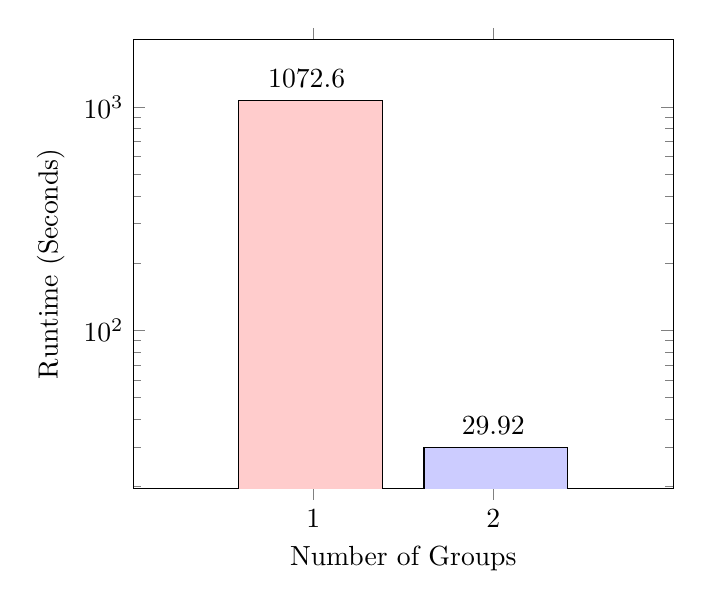
\begin{tikzpicture}
	\begin{axis}[ybar, ymode=log, ymax=2000, xmin=0, xmax=3, xtick={1,2}, xlabel=Number of Groups, ylabel=Runtime (Seconds)]
		\addplot[fill=red!20, bar width=0.8] coordinates {(1.4, 1072.6)};
		\addplot[fill=blue!20, bar width=0.8]  coordinates {(1.6, 29.92)};
	\end{axis}
	\node at (2.2,5.2){1072.6};
	\node at (4.57, 0.79){29.92};
\end{tikzpicture}
\caption{Runtimes for a 18 bus 12 charger scenario at a 0.13\% gap}
\label{fig:results:groupResults}
\end{figure}
 
\subsection{Effects of defragmentation}
This paper also addresses the operational preference to consolidate charge sessions when possible. This section demonstrates the effectiveness of the defragmentation method given in Section \ref{sec:defragmentation} and how consolidation affects the monthly cost. In Section \ref{sec:defragmentation}, the threshold for defragmentation is given by the minimum allowable energy per charge session. In this section we compare two 40 bus 7 charger scenarios where the first contains results without defragmentation and the second consolidates charge sessions so that each session delivers at least 30 kWh. The results for each session are presented in Figs. \ref{fig:results:noFragmentationChargeLimit} and \ref{fig:results:defragmentedChargeLimit} where the color of $i,j$ element of a figure represents the charge rate for bus $i$ during time $j$. Note how Fig. \ref{fig:results:noFragmentationChargeLimit} contains {\it many} small an inconsequential charge sessions and requires each bus to charge each time it enters the station. In comparison, Fig. \ref{fig:results:defragmentedChargeLimit} contains only a handful of charge sessions so that each bus only need charge 4 -- 5 times throughout the day.  
\par Furthermore, Fig. \ref{fig:results:defragmentationCostProTime} demonstrates that despite the additional constraints associated with consolidation, the monthly cost remains consistent over a large window of thresholds. As the minimum allowable energy per session increases, the number of binary variables in the defragmentation problem increases, resulting in significant runtimes for the defragmentation problem as shown in Fig. \ref{fig:results:defragmentationTimeProTime}. However, because buses are divided into groups prior to defragmentation, the smaller groups decrease the computational complexity for defragmentation so that larger consolidation thresholds can be applied in a scalable manner. 
\begin{figure*}
\begin{tikzpicture} 
\begin{axis}[colorbar, ChargeSessionImage, width=7.2in, height=3in, point meta min=0, point meta max=350, xmin=0.5, xmax=4320.5, xtick={540, 1080, 1620, 2160, 2700, 3240, 3780, 4320}, xticklabels={3:00, 6:00, 9:00, 12:00, 15:00, 18:00, 21:00, 0:00}, ymin=0.5, ymax=40.5]
\addplot [forget plot] graphics [xmin=0.5, xmax=4320.5, ymin=0.5, ymax=40.5] {media/11_results/defragmentedChargeLimit-1.png}; 
\end{axis} 
\end{tikzpicture}
\caption{Routes with De-Fragmentation}
\label{fig:results:defragmentedChargeLimit}
\end{figure*}

\begin{figure*}
\begin{tikzpicture} 
\begin{axis}[colorbar, ChargeSessionImage, width=7.2in, height=3in, point meta min=0, point meta max=350, xmin=0.5, xmax=4320.5, xtick={540, 1080, 1620, 2160, 2700, 3240, 3780, 4320}, xticklabels={3:00, 6:00, 9:00, 12:00, 15:00, 18:00, 21:00, 0:00}, ymin=0.5, ymax=40.5]
\addplot [forget plot] graphics [xmin=0.5, xmax=4320.5, ymin=0.5, ymax=40.5] {media/11_results/noFragmentationChargeLimit-1.png}; 
\end{axis} 
\end{tikzpicture}
\caption{Routes without De-Fragmentation}
\label{fig:results:noFragmentationChargeLimit}
\end{figure*}
 
\begin{figure}
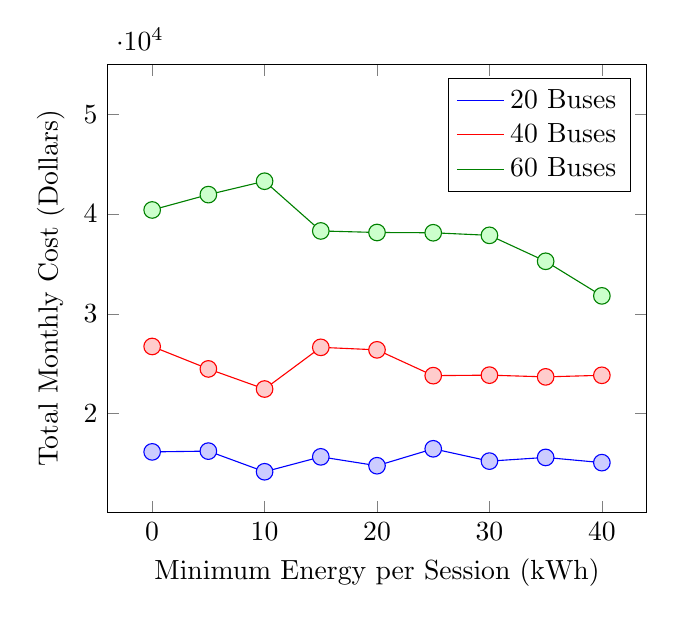
\begin{tikzpicture}
\begin{axis}[xlabel=Minimum Energy per Session (kWh), ylabel=Total Monthly Cost (Dollars), ymax=55000, legend pos=north east]
	\addplot[blue] coordinates {
		(0, 16183.79)   
	  (5, 16260.98)  
		(10,14194.10)  
		(15,15686.16)  
		(20,14798.53)  
		(25,16492.56)  
		(30,15259.19)  
		(35,15628.38)  
		(40,15106.82)};
\addplot[red] coordinates {
		(0, 26738.71)
		(5, 24491.03)
	  (10,22476.88)
		(15,26650.71)
		(20,26400.31)
		(25,23816.91)
		(30,23866.55)
		(35,23693.25)
		(40,23851.78)};
\addplot[green!50!black] coordinates {
		(0, 40405.72)
		(5, 41942.45)
	  (10,43284.09)
		(15,38304.96)
		(20,38150.28)
		(25,38122.51)
		(30,37864.79)
		(35,35268.11)
		(40,31805.12)};

\addplot[blue!20, draw=blue, only marks, mark size=3pt] coordinates {
		(0, 16183.79)  
		(5, 16260.98)  
	  (10,14194.10)  
		(15,15686.16)  
		(20,14798.53)  
		(25,16492.56)  
		(30,15259.19)  
		(35,15628.38)   
		(40,15106.82)};
\addplot[red!20, draw=red, only marks, mark size=3pt] coordinates {
	(0, 26738.71)  	
	(5, 24491.03)  	
	(10,22476.88)   
	(15,26650.71)  	
	(20,26400.31)  	
	(25,23816.91)  	
	(30,23866.55)  	
	(35,23693.25)  	
	(40,23851.78)};	
\addplot[green!20, draw=green!50!black, only marks, mark size=3pt] coordinates {
	(0, 40405.72)  
	(5, 41942.45)  
	(10,43284.09)  
	(15,38304.96)  
	(20,38150.28)  
	(25,38122.51)  
	(30,37864.79)  
	(35,35268.11)  
	(40,31805.12)};

\legend{20 Buses, 40 Buses, 60 Buses} 
\end{axis}
\end{tikzpicture}
\caption{Cost comparison of different degragmentation thresholds in a pro-time optimization scheme.}
\label{fig:results:costDefragmentationProTime}
\end{figure}

\begin{figure}\centering
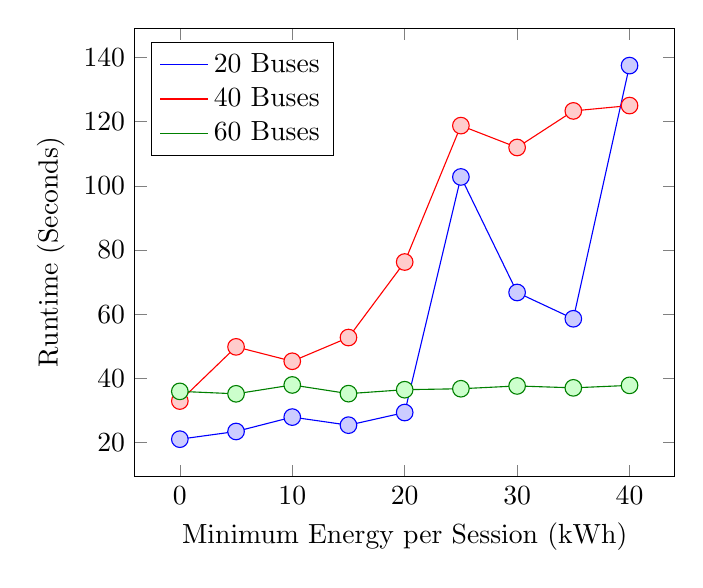
\begin{tikzpicture}
\begin{axis}[xlabel=Minimum Energy per Session (kWh), ylabel=Runtime (Seconds), legend pos=north west]
	\addplot[blue] coordinates {
		(0, 21.00)
		(5, 23.40)
	  (10,27.89)
		(15,25.37)
		(20,29.31)
		(25,102.78)
		(30,66.75)
		(35,58.55)
		(40,137.51)}; 
\addplot[red] coordinates {
		(0, 32.89)
		(5, 49.79)
	  (10,45.30)
		(15,52.70)
		(20,76.25)
		(25,118.79)
		(30,111.97)
		(35,123.37)
		(40,125.04)}; 
\addplot[green!50!black] coordinates {
		(0, 35.91)
		(5, 35.15)
	  (10,37.91)
		(15,35.20)
		(20,36.43)
		(25,36.73)
		(30,37.60)
		(35,37.01)
		(40,37.78)}; 
\addplot[blue!20, draw=blue, only marks, mark size=3pt] coordinates {
		(0, 21.00)
		(5, 23.40)
	  (10,27.89)
		(15,25.37)
		(20,29.31)
		(25,102.78)
		(30,66.75)
		(35,58.55)
		(40,137.51)}; 
\addplot[red!20, draw=red, only marks, mark size=3pt] coordinates {
		(0, 32.89)
		(5, 49.79)
	  (10,45.30)
		(15,52.70)
		(20,76.25)
		(25,118.79)
		(30,111.97)
		(35,123.37)
		(40,125.04)}; 
\addplot[green!20, draw=green!50!black, only marks, mark size=3pt] coordinates {
		(0, 35.91)
		(5, 35.15)
	  (10,37.91)
		(15,35.20)
		(20,36.43)
		(25,36.73)
		(30,37.60)
		(35,37.01)
		(40,37.78)}; 
\legend{20 Buses, 40 Buses, 60 Buses}		
\end{axis}
\end{tikzpicture}
\caption{Comparison of runtime for the uncontested and contested scenarios over different de-fragmentation criteria}
\label{fig:results:defragmentationTimeProTime}
\end{figure}

\subsection{Scalability}
In this section, we consolidate what we have learned in the previous sections to demonstrate how the proposed framework can be used to compute a scalable and cost effective solution for large numbers of buses. This section focuses on a scenario with a minimum energy per session of 20 kWh, a relaxed gap for the charger assignment solution, and a single group.
\par The results given in Fig. \ref{fig:results:scalabilityRuntimes} show a runtime that generally increases by one second per bus from 10 to 110 buses.  One would expect the runtime to increase at least on the order of $O(n^2)$ for a globally optimal solution because of the coupling between bus variables. The fact that the proposed method appears linear on the given range indicates a scalable solution. 
\par Generally, one would also expect such savings to come with significant increases to the monthly cost. The results in Fig. \ref{fig:results:scalabilityCosts} however demonstrate how the proposed solution yields a quasi-linear increase of approximately \$404.10 dollars per bus per month. 
\begin{figure}\centering
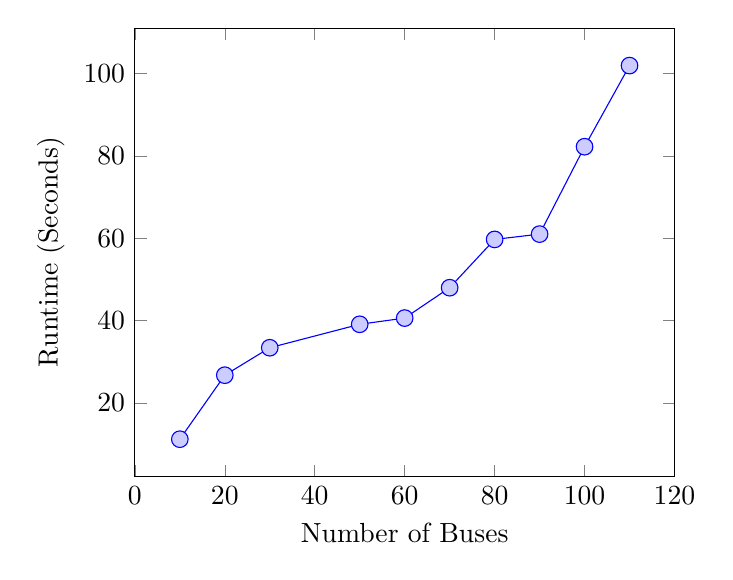
\begin{tikzpicture}
\begin{axis}[xlabel=Number of Buses, ylabel=Runtime (Seconds), legend pos=north west]
	\addplot[blue] coordinates {
		(10, 11.18)   
	  (20, 26.74)  
		(30, 33.41)  
		(50, 39.11)  
		(60, 40.62)  
		(70, 48.00)  
		(80, 59.74)  
		(90, 61.03)
		(100, 82.27)
		(110, 101.99)}; 
\addplot[blue!20, draw=blue, only marks, mark size=3pt] coordinates {
		(10, 11.18)   
	  (20, 26.74)  
		(30, 33.41)  
		(50, 39.11)  
		(60, 40.62)  
		(70, 48.00)  
		(80, 59.74)  
		(90, 61.03)
		(100, 82.27)
		(110, 101.99)};
\end{axis}
\end{tikzpicture}
\caption{Runtime comparison for different numbers of buses}
\label{fig:results:scalabilityRuntimes}
\end{figure}

\begin{figure}
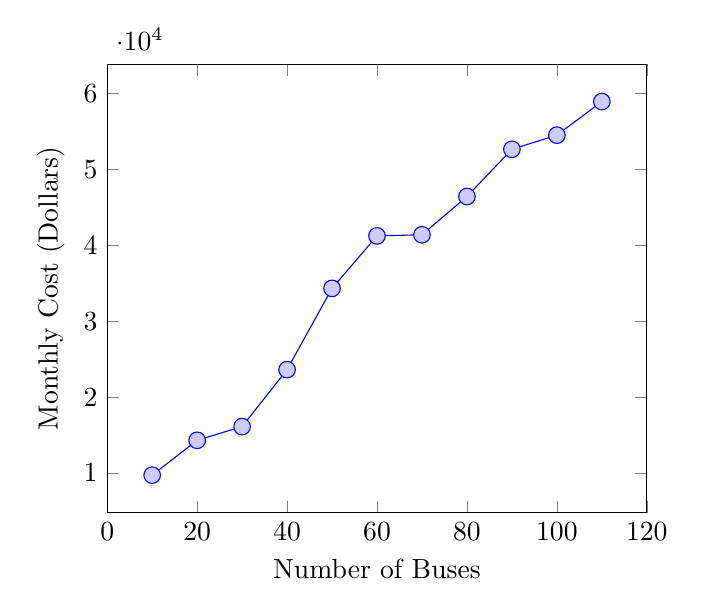
\begin{tikzpicture}
\begin{axis}[xlabel=Number of Buses, ylabel=Monthly Cost (Dollars), legend pos=north west]
	\addplot[blue] coordinates {
		(10, 9724.43)   
	  (20, 14312.58)  
		(30, 16113.51)  
		(40, 23617.81)
		(50, 34317.80)  
		(60, 41226.07)  
		(70, 41374.21) 
		(80, 46412.54)  
		(90, 52628.26)
		(100, 54490.15) 
		(110, 58912.91)}; 
\addplot[blue!20, draw=blue, only marks, mark size=3pt] coordinates {
		(10, 9724.43)   
	  (20, 14312.58)  
		(30, 16113.51)  
		(40, 23617.81)
		(50, 34317.80)  
		(60, 41226.07)  
		(70, 41374.21)  
		(80, 46412.54)  
		(90, 52628.26)
		(100, 54490.15) 
		(110, 58912.91)}; 
\end{axis}
\end{tikzpicture}
\caption{Cost comparison for different numbers of buses}
\label{fig:results:scalabilityCosts}
\end{figure}

	
	

\section{Conclusions}
In summary, this paper proposes a method to compute cost-oriented charge schedules for large numbers of battery electric buses by dividing the charge problem into several sub-problems which focus on energy placement and group separation, charge session length and assignment, and cost optimization. The proposed method has been shown to scale as both the runtime and monthly cost increase linearly with the number of buses. 
\par Furthermore, because the proposed method contains a number of sub-problems, setting the optimization criteria for each sub-problem gives the user flexibility so that the proposed method can be adapted to solve a variety of scenarios and optimization preferences.

\onecolumn
\newcommand\mybar{\kern1pt\rule[-\dp\strutbox]{.8pt}{\baselineskip}\kern1pt}
\newcommand{\coloredhline}{\arrayrulecolor{gray!20} \hline \\[0.01in]\arrayrulecolor{black}}
\newcommand{\myendline}{\\ \coloredhline}
\begingroup
\fontsize{8pt}{10pt}\selectfont
\label{tab:paperVariables}
\centering
\begin{supertabular}{b{0.05\textwidth} m{0.25\textwidth} m{0.06\textwidth} m{0.05\textwidth} m{0.25\textwidth} m{0.06\textwidth}}
	\toprule%----------------------------------------------------------------------------
	\textbf{Variable} & \textbf{Description} & \textbf{Range} & \textbf{Variable} & \textbf{Description} & \textbf{Range}\\
	\toprule%-----------------------------------------------------------------------------
	\multicolumn{6}{l}{Indices} \myendline
	i & Bus index     & $\mathbb{N}$ & j & Time Index & $\mathbb{N}$\\ \myendline
	k & Charger index & $\mathbb{N}$ & r & Route Index \\ \myendline
  m & group index   & $\mathbb{N}$ &   &             \\[0.15in]
	\hline \\[-5pt]
	\multicolumn{6}{l}{Optimal Solution | Formulation} \\[-9pt]\myendline
	$n_{\text{bus}}$&\parbox{0.2\textwidth}{The number of buses in the optimization framework.}                                                           & $\mathbb{Z}$            & $n_{\text{time}}$                      &\parbox{0.2\textwidth}{ The number of time indices in a day.                                                                                 }      & $\mathbb{Z}^+$ \\\myendline
	$b_{p(i,j)}$   & \parbox{0.2\textwidth}{The average power consumed by bus $i$ during time period $j$.}                                                                              & $\mathbb{R}$           & $t_j$         &\parbox{0.2\textwidth}{ The time at time index $j$. This paper also refers to the period of time from $t_j$ to $t_{j+1}$ as ``period $t_j$''.}      & $\mathbb{R}$\\\myendline 
	$\bm{b}$       & \parbox{0.2\textwidth}{A vector containing each value for $b_{p(i,j)}$.}                                                                                          & $\mathbb{R}^{n_{\text{bus}}\cdot n_{\text{time}}}$           & 	$\mathcal{\tilde{A}}$  & \parbox{0.2\textwidth}{The complement of $\mathcal{A}$.}                                                                        & $i\times j$\\\myendline 
	$\mathcal{A}$  & \parbox{0.2\textwidth}{The set of all $i\times j$ elements where bus $i$ can charge at time index $j$}                                  & $i\times j$             & $p_{\text{max}}$ &\parbox{0.2\textwidth}{The maximum power a bus charger can deliver to a bus in kW. This paper assumes a value of 350 for most examples and results.} & $\mathbb{R}^+  $\\[0.5in]
	\hline \\[-0.07in]
	\multicolumn{6}{l}{Optimal Solution | Battery} \\[-9pt] \myendline
	$h_{\text{min}}$ & The minimum allowable state of charge                           & $\left ( 0,h_{\text{max}} \right )$                & $h_{\text{max}}$  & The maximum state of charge                                                   & $\mathbb{R}^+$                                     \\ \myendline 
	$\eta_i$         & The beginning state of charge for bus $i$                       & $\left ( h_{\text{min}}, h_{\text{max}} \right )$  & $h(ij)$           & The state of charge for bus $i$ at time $t_j$. & $\left ( h_{\text{min}}, h_{\text{max}} \right )$\\ \myendline
	$\Delta T$       & The change in time from $t_j$ to $t_{j+1}$                      &$\mathbb{R}^+ $  & $\bm{h}$             & A vector containing all state of charge values.                                        & $\mathbb{R}_+^{n_{\text{bus}}\cdot n_{\text{time}}}$                                   \\ \myendline
	$\delta(ij)$     & The battery discharge for bus $i$ during time period $j$.               & $\mathbb{R}_+$                                     & $h(i,\text{end})$& Bus $i$'s final state of charge.                                              & $\left ( h_{\text{min}}, h_{\text{max}} \right )$\\[0.3in]
	\hline \\[-0.07in]
	\multicolumn{6}{l}{Optimal Solution | Cumulative Load Management} \\[-9pt] \myendline 
	$n_{\text{charger}}$             & The time index for the start of bus $i$'s $j^{\text{th}}$ stop                                                    & $\mathbb{Z}_+$                   & $p_c(j)$            & The average power consumed by all buses during time period $j$. & $\mathbb{R}$                    \\ \myendline
	$\bm{p_c}$                       & A vector containing all values of $p_c(j)$.                                                                       & $\mathbb{R}_{+}^{n_{\text{time}}}$                   & $J_{\text{thrash}}$          & A secondary objective function which penalizes multiple plug-in instances per charge session.& $\mathbb{R}_+$ \\ \myendline
	$g(i,j)$                         & A slack variable used to compute the absolute value of $\lvert b_{p(i,j)} - b_{p(i,j-1)}\rvert$ & $\mathbb{R}_+$& & &                \\[0.3in] 
	\hline \\[-0.07in]
	\multicolumn{6}{l}{Optimal Solution | Objective}  \\[-9pt] \myendline
	$\mu_{\text{e-on}}$         & On-Peak Energy Rate                                                            & $\mathbb{R}_+$                                & $\mu_{\text{e-off}}$       & Off-Peak Energy Rate                                                                                     & $\mathbb{R}_+$                 \\ \myendline
	$\mu_{\text{p-on}}$         & On-Peak Demand Power Rate                                                      & $\mathbb{R}_+$                                & $\mu_{\text{p-all}}$       & Facilities Power Rate                                                                                    & $\mathbb{R}_+$                 \\ \myendline
	$\mathcal{S}_{\text{on}}$   & The set of on-peak time indices                                                & \scalebox{0.9}{$\{1,...,n_{\text{time}}\}$}   & $p_{\text{demand}}$        & Maximum average power during on-peak periods                                                             & $\mathbb{R}$                 \\ \myendline
	$p_{\text{facilities}}$     & Maximum average power over all time instances.                                 & $\mathbb{R}_+$                                & $p_t(j)$                   & The total average power co nsumed by both the bus chargers and the uncontrolled loads.                    & $\mathbb{R}_+^{n_{\text{time}}}$  \\ \myendline
	$u(j)$                      & The average power over time $j$ consumed by the uncontrolled loads             & $\mathbb{R}_+^{n_{\text{time}}}$            & $\bm{p}_t$                 & a vector containing $p_t(i)$ for all $i$.                                                                  & $\mathbb{R}_+^{n_{\text{time}}}$ \\ \myendline 
	$e_{\text{on}}$             & The total amount of energy consumed by the bus chargers and uncontrolled loads during off-peak hours.& $\mathbb{R}_+$                              & $e_{\text{off}}$             & The total energy consumed by the bus chargers and uncontrolled loads during on-peak hours.               & $\mathbb{R}_+$ \\ \myendline 
	$J_{\text{cost}}$           & The section of the objective function pertaining to the fiscal expense of charging buses. & $\mathbb{R}$                & $J_{\text{all}}$               & The expression for the complete objective function. & $\mathbb{R}$ \\[0.3in]
	\hline \\[-0.07in] 
	\multicolumn{6}{l}{Scalability}  \\[-9pt] \myendline
	$n_{\text{group}}$         & The number of groups in which to divide the buses and available chargers in preparation for the $p_4$, $p_5$, and $p_6$.                                                           & $\mathbb{Z}_+$                                & $n_{\text{charger}}^m$      & The number of chargers assigned to group $m$.             & $\mathbb{Z}_+$ \myendline
  $n_{\text{bus}}^m$         & The number of buses in group $m$.                                                                                      &$\mathbb{Z}_+$ & $p(j,m)$ & The total power used during time index $j$ by all buses in group $m$. & $\mathbb{R}_+$      \myendline
  $\beta(i,m)$               & A binary selector variable which is one when bus $i$ is in gropu $m$ and zero otherwise.                               &$\{0,1\}$      & $n_{\text{charger}}^m$ & The number of chargers assigned to group $m$            & $\mathbb{Z}_+$      \myendline
  $\phi(i,i')$                  & The inner product of the optimal charge schedules for buses $i$ and $i'$ respectively.                                 &$\mathbb{R}_+$&$v(i,i',g)$ & A variable that is $w(i,i')$ when buses $i$ and $i'$ are in group $g$ and zero otherwise. & $\mathbb{Z}_+$    \myendline
  $M_s$                      & The maximum value for $\phi(i,i')$.                                                                                       &$\mathbb{R}_+$&$J_{\text{select}}$ & The objective function for the group-selection problem & $\mathbb{R}_+$ \\[0.3in]
	\hline \\[-0.07in] 
	\multicolumn{6}{l}{De-Fragmentation}  \\[-9pt] \myendline
	$\theta(i,r)$& A binary variable which is one when charge session $r$ from bus $i$ will be used in a defragmented solution. & $\{0,1\}$ & $\rho(i,r)$ & A vector whose elements are equal to $\Delta T$ during time indices when bus $i$ is charging during charge session $r$ and zero otherwise.  & $\mathbb{R}^{n_{\text{time}}}$\\ \myendline
  $\psi(i,j)$& The minimum allowable energy delivered to bus $i$ during charge session $r$ where the session in question is considered ``active''. & $\mathbb{R}$& $\omega$	& The minimum allowable energy for any charge session. & $\mathbb{R}$ \\ \myendline
	$e_{\text{max}}$ & The maximum allowable energy delivered in any session.                                                                        & $\mathbb{R}$& & & \\[0.3in] 
	\hline \\[-0.07in]
	\multicolumn{6}{l}{Charge Schedules}  \\[-9pt] \myendline
	$a(i,r)$ & The beginning of the allowable charge interval for bus $i$'s $r^{\text{th}}$ charge session. & $\mathbb{R}_+$ & $b(i,r)$ & The commanded start time for bus $i$'s $r^{\text{th}}$ charge session& $\mathbb{N}$\\ \myendline
	$f(i,r)$ & The commanded end time for bus $i$'s $r^{\text{th}}$ charge session. & $\mathbb{R}_+$ & $d(i,r)$ & The end time of the allowable charge interval for bus $i$'s $r^{\text{th}}$ charge session. & $\mathbb{R}_+$ \\\myendline
	$\sigma(i,r,k)$& A selector variable which is one when bus $i$ charges at charger $k$ for session $r$. & $\{0,1\}$ & $M$ & The number of seconds in a day & $\mathbb{Z}_+$ \\ \myendline
	\scalebox{0.8}{$l(i,r,i',r')$} & A selector variable which is one when bus $i$ charges before bus $i'$ during the $r$ and $r'$ sessions respectively. & $\{0,1\}$& & & \\[0.3in]
	\hline \\[-0.07in]	
	\multicolumn{6}{l}{Optimizing Charge Schedules}  \\[-9pt] \myendline
	$c(s,i,r)$ & The start time for bus $i$'s $r^{\text{th}}$ charge session.  & $\mathbb{R}$ & $c(f,i,r)$& The stop time for bus $i$'s $r^{\text{th}}$ charge session. & $\mathbb{R}$ \\ \myendline
	$c(a,i,r)$ & The arrival time of bus $i$ for charge session $r$.           & $\mathbb{R}$ & $c(d,i,r)$& The departure time for bus $i$ after having completed the $r^{\text{th}}$ charge session& $\mathbb{R}$ \myendline
	$J_{\text{window}}$ & The loss function which drives charge windows to the desired length.& $\mathbb{R}$ & & & \\[0.3in]
	\hline \\[-0.07in]
	\multicolumn{6}{l}{Multi-Rate Charging}  \\[-9pt] \myendline
	$x(i,j)$ & The final charge schedule for bus $i$ at time $j$, yielding the power at which bus $i$ will charge.& $\mathbb{R}_+$ & $z(j)$ & The total power used by all buses at time $j$. $\mathbb{R}_+$ \\ \myendline
  $\gamma(i,d)$ & A binary vector which is one at all time steps where bus $i$ charges during charge session $d$. &$\{0,1\}^{n_{\text{time}}}$& $e(i,r)$               &The amount of energy to be delivered to bus $i$ during charge session $r$.        &$\mathbb{R}_+$            \\ \myendline
  $J_{\text{multi-rate}}$ & The objective function over which we minimize to solve the multi-rate section of the bus charge problem. & $R_+$& &  &             \\[0.3in] 
	\hline \\[-0.07in]
	%
\end{supertabular}
\endgroup 


\begin{adjustwidth}{-\extralength}{0cm}
%\printendnotes[custom] % Un-comment to print a list of endnotes

\reftitle{Referencess}

% Please provide either the correct journal abbreviation (e.g. according to the “List of Title Word Abbreviations” http://www.issn.org/services/online-services/access-to-the-ltwa/) or the full name of the journal.
% Citations and References in Supplementary files are permitted provided that they also appear in the reference list here. 

%=====================================
% References, variant A: external bibliography
%=====================================
 \bibliography{references.bib}

%=====================================
% References, variant B: internal bibliography
%=====================================
% \begin{thebibliography}{999}
% % Reference 1
% \bibitem[Author1(year)]{ref-journal}
% Author~1, T. The title of the cited article. {\em Journal Abbreviation} {\bf 2008}, {\em 10}, 142--149.
% % Reference 2
% \bibitem[Author2(year)]{ref-book1}
% Author~2, L. The title of the cited contribution. In {\em The Book Title}; Editor 1, F., Editor 2, A., Eds.; Publishing House: City, Country, 2007; pp. 32--58.
% % Reference 3
% \bibitem[Author3(year)]{ref-book2}
% Author 1, A.; Author 2, B. \textit{Book Title}, 3rd ed.; Publisher: Publisher Location, Country, 2008; pp. 154--196.
% % Reference 4
% \bibitem[Author4(year)]{ref-unpublish}
% Author 1, A.B.; Author 2, C. Title of Unpublished Work. \textit{Abbreviated Journal Name} year, \textit{phrase indicating stage of publication (submitted; accepted; in press)}.
% % Reference 5
% \bibitem[Author5(year)]{ref-communication}
% Author 1, A.B. (University, City, State, Country); Author 2, C. (Institute, City, State, Country). Personal communication, 2012.
% % Reference 6
% \bibitem[Author6(year)]{ref-proceeding}
% Author 1, A.B.; Author 2, C.D.; Author 3, E.F. Title of presentation. In Proceedings of the Name of the Conference, Location of Conference, Country, Date of Conference (Day Month Year); Abstract Number (optional), Pagination (optional).
% % Reference 7
% \bibitem[Author7(year)]{ref-thesis}
% Author 1, A.B. Title of Thesis. Level of Thesis, Degree-Granting University, Location of University, Date of Completion.
% % Reference 8
% \bibitem[Author8(year)]{ref-url}
% Title of Site. Available online: URL (accessed on Day Month Year).
% \end{thebibliography}

% If authors have biography, please use the format below
%\section*{Short Biography of Authors}
%\bio
%{\raisebox{-0.35cm}{\includegraphics[width=3.5cm,height=5.3cm,clip,keepaspectratio]{Definitions/author1.pdf}}}
%{\textbf{Firstname Lastname} Biography of first author}
%
%\bio
%{\raisebox{-0.35cm}{\includegraphics[width=3.5cm,height=5.3cm,clip,keepaspectratio]{Definitions/author2.jpg}}}
%{\textbf{Firstname Lastname} Biography of second author}

% For the MDPI journals use author-date citation, please follow the formatting guidelines on http://www.mdpi.com/authors/references
% To cite two works by the same author: \citeauthor{ref-journal-1a} (\citeyear{ref-journal-1a}, \citeyear{ref-journal-1b}). This produces: Whittaker (1967, 1975)
% To cite two works by the same author with specific pages: \citeauthor{ref-journal-3a} (\citeyear{ref-journal-3a}, p. 328; \citeyear{ref-journal-3b}, p.475). This produces: Wong (1999, p. 328; 2000, p. 475)

%%%%%%%%%%%%%%%%%%%%%%%%%%%%%%%%%%%%%%%%%%
%% for journal Sci
%\reviewreports{\\
%Reviewer 1 comments and authors’ response\\
%Reviewer 2 comments and authors’ response\\
%Reviewer 3 comments and authors’ response
%}
%%%%%%%%%%%%%%%%%%%%%%%%%%%%%%%%%%%%%%%%%%
\end{adjustwidth}
\end{document}

